\documentclass[journal,twoside]{IEEEtran}
\usepackage{graphicx}
\usepackage{url}
%\usepackage{slashbox}
\usepackage{amsmath}
\usepackage{enumerate}
%\usepackage{algorithm}
\usepackage{cite}
%\usepackage{algorithmic}
\usepackage{multirow}
\usepackage{subfigure}
\usepackage{diagbox}
\usepackage{float}
\usepackage{booktabs}
\usepackage{epstopdf}
\usepackage{subfigure}
\usepackage{multicol}
\usepackage{txfonts}
\usepackage{bm}
\usepackage{xr}
\usepackage{makecell}
\usepackage{changepage}
\usepackage{threeparttable}
\usepackage{bbding}
\usepackage[linesnumbered,ruled,vlined]{algorithm2e}


%\usepackage{slashbox}
%\usepackage{diagbox}
%\usepackage{tabularx}
\usepackage{color}
\definecolor{blue}{rgb}{0,0,1}



% correct bad hyphenation here
\hyphenation{op-tical net-works semi-conduc-tor}

\begin{document}
\title{Advanced 3D Wind Farm Layout Optimization Framework via Power-Law Perturbation-based Genetic Algorithm}
%\author{
%    Jiaru Yang,~\IEEEmembership{Student Member,~IEEE} Yaotong Song, Jun Tang, Weiping Ding,~\IEEEmembership{Senior Member,~IEEE}, Zhenyu Lei, and Shangce Gao,~\IEEEmembership{Senior Member,~IEEE}
%    \thanks{\quad This research was partially supported by the Japan Society for the Promotion of Science (JSPS) KAKENHI under Grant JP23K24899, and Japan Science and Technology Agency (JST) Support for Pioneering Research Initiated by the Next Generation (SPRING) under Grant JPMJSP2145. We sincerely thank to China Huaneng Group for generously providing data.}
%    \thanks{\quad J.~Yang, Y.~Song, Z.~Lei and S.~Gao are with the Faculty of Engineering, University of Toyama, Toyama-shi, 930-8555, Japan. (E-mail: d2272009@ems.u-toyama.ac.jp; m23c1048@ems.u-toyama.ac.jp; leizg@eng.u-toyama.ac.jp; gaosc@eng.u-toyama.ac.jp)}
%    \thanks{\quad J.~Tang is with the Wicresoft Co Ltd, 13810 SE Eastgate Way, Bellevue, WA 98005, USA. (E-mail: juntang@wicresoft.com)}
%    \thanks{\quad W.~Ding is with the School of Artificial Intelligence and Computer Science, Nantong University, Nantong, China and also with the Faculty of Data Science, City University of Macau, Macau, China. (E-mail: ding.wp@ntu.edu.cn)}
%}

\maketitle
% make the title area


\begin{abstract}
The modeling and optimization of wind farm layouts can effectively reduce the wake effect between turbine units, thereby enhancing the expected output power and avoiding negative influence. Traditional wind farm optimization often uses idealized wake models, neglecting the influence of wind shear at different elevations, which leads to a lack of precision in estimating wake effects and fails to meet the accuracy and reliability requirements of practical engineering. To address this, we have constructed a three-dimensional 3D wind farm optimization model that incorporates elevation, utilizing a 3D wake model to better reflect real-world conditions. We aim to assess the optimization state of the algorithm and provide strong incentives at the right moments to ensure continuous evolution of the population. To this end, we propose an evolutionary adaptation degree-guided genetic algorithm based on power-law perturbation (PPGA) to adapt multidimensional conditions. We select the offshore wind power project in Nantong, Jiangsu, China as a study example and compare PPGA with other well-performing algorithms under this practical project. Based on the actual wind condition data, the experimental results demonstrate that PPGA can effectively tackle this complex problem and achieve the best power efficiency.
\end{abstract}

\begin{IEEEkeywords}
	Offshore wind farm, 3D wake model, Power-law perturbation, Meta-heuristic, China's southeastern coast
\end{IEEEkeywords}

\IEEEpeerreviewmaketitle


\section{Introduction}
    \IEEEPARstart{T}{o} address the climate crisis and achieve the ambitious goal of carbon neutrality, optimizing the energy mix and discovering sustainable, clean, low-carbon, and cost-effective alternative energy sources have become a common goal of humankind \cite{liu2023climate}. Over the past 20 years, wind energy has emerged as the most competitive clean energy source. By 2022, the total installed wind power capacity is projected to reach 906 GW, with a steadily accelerating growth rate \cite{wiser2023land}.  
    
    At this stage, onshore wind power retains the primary focus of development, holding the largest share in the energy landscape. Nonetheless, in recent years, expectations for onshore wind power and its growth rates have begun to decline. In regions like China, characterized by a densely populated coastal plain with soaring land costs, the future return on investment for onshore wind farms faces challenges. Furthermore, the impact of climate change has led to a long-term trend of declining wind speeds in traditionally wind-rich areas, such as Inner Mongolia, raising concerns about the future viability of onshore power generation \cite{xia2023potential}. \textcolor{blue}{Offshore wind power emerges as a promising solution to several of these challenges in wind energy development. As installation technology advances and maintenance costs decrease, the advantages of offshore wind power are becoming more evident.} Research indicates that the total wind resource potential off China's eastern coast is 5.4 times the current coastal electricity demand \cite{sherman2020offshore}. Fig.~\ref{nantong} shows an offshore wind farm project in Nantong, Jiangsu, China. Similarly, developed countries with extensive coastlines, such as the United States and Europe, are increasingly shifting their investments and policies towards offshore power generation.    
    \begin{figure}[!t]
    	\centering
    	%\setlength{\abovecaptionskip}{-0.2cm}
    	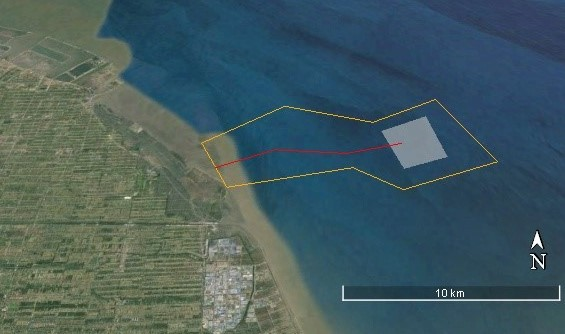
\includegraphics[width=\linewidth,scale=1]{nantong1.jpg}
    	\caption{The location of Nantong offshore wind farm No. 1 project.}
    	\label{nantong}
    	\vspace{-5 mm}
    \end{figure}

    To maximize the conversion rate of clean energy, researchers have delved into the efficiency optimization and cost planning of wind farms. The holistic framework for optimizing wind power presents a multi-disciplinary challenge, encompassing wind turbine design, wind farm layout optimization, cable configuration, and other pertinent factors. The precise layout of wind turbines takes center stage in enhancing the annual energy output. By arranging the position in a rational manner, we can mitigate the mutual interference of wake streams between turbines, consequently augmenting the overall power generation capacity \cite{howland2022operating}. \textcolor{blue}{Poor turbine arrangement exacerbates wake effects, where reduced wind speed lowers downstream turbine output and uneven wind loads increase fatigue risk \cite{howland2022collective,kitzing2020multifaceted}.} 
    
    \textcolor{blue}{The challenge of this complex system lies in balancing factors like wake effects, turbine spacing, terrain complexity, and obstacles to reduce energy losses and maximize power output \cite{tao2020nonuniform}.} The wake effect should be carefully considered in the design of wind farms in order to avoid negative impacts. Nowadays, the mainstream wake models are semi-empirical constructive models, such as the Jensen model \cite{shakoor2016wake} , the Gaussian model \cite{yu2023reinforcement}, and so on. Bastankhah et al. \cite{bastankhah2014new} employ the principle of momentum and mass conservation to calculate the wake velocity deficit based on the Frandsen model. The wind profiles and power estimates obtained from this 2D model are in agreement with the wind tunnel test results. In~\cite{zhang2020novel}, Zhang et al. train this dynamic wake model to capture high-fidelity wake features with the help of deep learning for numerical simulation of wake. This study is an attempt to use machine learning for addressing complex energy-related challenges. Ling et al. \cite{ling2023three} proposes a simple and efficient three-dimensional wake model for accurately predicting the wake effects of wind turbines, considering wind shear, anisotropic wake expansion, and mass loss caused by shear. This work highlights the importance of a 3D wake model in providing a more realistic representation of wake behavior, enabling more accurate power generation predictions, and enhancing layout optimization and wake control strategies. In recent years, scholars have proposed a variety of high-fidelity wake models, emphasizing the importance of scientific and accurate wake modeling in constructing wind farm optimization models.
    
    These models can accurately reflect the wake effect among turbines. Therefore, optimizing their layout to minimize the influence of the wake effect becomes crucial. Evolutionary algorithms have been proven to be an effective and low-cost approach for computationally large-scale, extreme multimodal constraint problems \cite{miikkulainen2021biological,tang2021review}. Since the first attempts to employ genetic algorithm (GA) \cite{mosetti1994optimization} to wind farm layout optimization, quite a number of improved GAs and model optimization studies have been developed. Gao et al. \cite{gao2016optimization} propose a two-dimensional parsimonious Jensen-Gaussian wake model, and develop a multi-population GA algorithm to optimize the layout model. Abdelsalam and Shorbagy \cite{abdelsalam2018optimization} use a binary GA with enhanced local search to attain the optimal solution for turbine siting. Along with the emergence of metaheuristic algorithms in recent years, a variety of more powerful metaheuristic methods have shown advantages in the field of wind farm optimization. Wang et al.\cite{wang2017differential} introduce a novel coding mechanism for the location of wind turbines by using differential evolution as an optimizer, thus reducing the dimensionality of the search space. The optimization method achieves a good performance in terms of computational cost and power output for a variety of wind scenarios. Lei et al.\cite{lei2023chaotic} develop a chaotic particle swarm optimizer that focuses on local exploitation, enhancing the properties of chaotic mapping to promote the search capability of the solution space. The optimizer shows more stable and powerful optimization performance under four complex wind conditions with different wind farm sizes.
    
    \textcolor{blue}{In wind farm layout optimization, the objective function often involves nonlinear and non-convex relationships, such as wake effects, terrain constraints, and variable wind conditions. GAs seamlessly integrate these constraints and handle trade-offs without requiring gradient information, making them particularly suitable for non-differentiable or discontinuous functions. Moreover, GAs excel in optimizing discrete problems like wind farm layouts, where solutions typically consist of discrete variables. They perform extensive searches across large search spaces while ensuring generated solutions remain feasible, effectively exploring the solution space to satisfy all constraints.} However, GAs also exhibit high randomness, especially in complex multimodal problems where they may become trapped in local optima. Early convergence of the population can result in evolutionary stagnation, preventing further improvement in solution quality \cite{wang2020multi,kirchner2024wind}. Therefore, we propose an evolutionary adaptation degree index to assess the optimization status of the population and decide when to intervene, aiding continued evolution. Previous studies have shown that power-law distributions are highly effective in modeling dynamic population systems and complex phenomena, owing to their ability to capture the heterogeneous and scale-free characteristics commonly observed in such systems \cite{holme2019rare}. Motivated by this, we propose a power-law perturbation-based genetic algorithm (PPGA) guided by an evolutionary adaptation degree. This approach improves upon the shortcomings of traditional heuristic algorithms, which tend to become trapped in local optima or converge prematurely when tackling complex optimization problems characterized by high dimensionality and nonlinearity. By incorporating power-law perturbation, PPGA introduces controlled randomness that enhances exploration and preserves population diversity, allowing the algorithm to adapt more effectively and evolve within complex solution spaces. When the evolutionary adaptation degree indicates insufficient progress, power-law perturbation is introduced to help the population escape local optima.
    
    Furthermore, to address the significant impact of terrain elevation and altitude variations on wind speed and direction that traditional two-dimensional modeling often neglects, we have introduced a 3D optimization framework incorporating altitude. Three-dimensional terrain modeling more accurately reflects the complexities of real-world environments, simulating wind flow under varying terrain conditions to more precisely predict the influence of each turbine's position on the overall wind farm. This precision is crucial for optimizing turbine layout, maximizing wind energy utilization, and reducing wake effects. This innovative 3D modeling approach not only offers higher theoretical accuracy and practicality but also provides new perspectives and tools for wind farm layout optimization. By integrating the three-dimensional characteristics of terrain and wake effects, we can develop more robust and efficient wind energy solutions, advancing renewable energy technology. Using the Nantong offshore wind power project as a case study, we test PPGA and seven other powerful algorithms under four real wind conditions and different numbers of wind turbines. PPGA achieves the best and most stable efficiency output in these simulations. The contributions can be concluded as follows: 
     \begin{itemize}
    	\item [1)]This study builds a 3D wind farm layout optimization model by incorporating altitude into the framework. To account for wake effects, a validated 3D Gaussian wake model is utilized to better approximate realistic conditions. 
    	\item [2)]We propose an evolutionary adaptation degree-guided genetic algorithm based on power-law perturbation (PPGA) to facilitate population evolution in continuously seeking optimal solutions within complex discrete search spaces. 
    	\item [3)]By using a realistic wind farm as an optimization example, we demonstrate the potential of the proposed method for engineering optimization. It can provide a reference for the future development of wind power along the southeast coast of China.
      \end{itemize} 
  
	The remainder sections are as follows: Section \ref{sec_3d_moding} introduces the framework of 3D wind farm layout optimization and high fidelity wake model. Section \ref{sec_PPGA} presents the motivation and the operating mechanism of PPGA. Section \ref{sec_experiment} reveals the experimental results on a practical instance considering constraints and non-uniform wind scenarios, validating the potential of PPGA in addressing wind farm layout optimization. Besides, the threshold analysis of evolutionary adaption degree and the discussion of stagnant optimization are also performed in this section. Section \ref{sec_conclusion} summarizes this work and provides an outlook for future industrial applications.

\section{Wind farm layout optimization framework}
\label{sec_3d_moding}
    This section presents a comprehensive introduction to the holistic optimization framework for 3D modeling of wind farm layouts. It encompasses the establishment of objective function and the construction of a 3D wake model. 
    \subsection{3D Wind Farm Layout Optimization Modeling}
    Previous studies have explored 3D frameworks, but they are limited by optimization techniques and the development of wake models. Huang et al. \cite{8571249} optimize both the horizontal layout and vertical hub height of wind turbines simultaneously through a nested loop approach, considering fatigue impacts and operational costs. However, this model relies on the traditional planar Jensen wake model, which does not fully account for constraints or the effects of non-uniform wind speeds. Tao et al.\cite{tao2020wind} propose a novel 3D wake model for wind farm layout optimization, while experimental cases are conducted under idealized planar conditions, neglecting the effects of real terrain. Developing a reliable framework that comprehensively integrates terrain, wind conditions, wake models, and constraints remains a critical challenge.
    
    \textcolor{blue}{To streamline computations, we adopt a discrete model for turbine placement within the available sea area, dividing it into a predefined grid with one turbine per grid cell. While most studies simplify the problem by assuming a flat surface, reducing it to a 2D model, we construct a 3D wind farm optimization model to better reflect real-world complexity scenarios \cite{hu2024wind}. As illustrated in Fig.~\ref{3dwind}, the model accounts for terrain elevation, where $r$ is the rotor radius, $h$ is the turbine height above sea level, and $z$ is the foundation elevation, making the absolute turbine center height $z+h$.}
    \begin{figure}[!t]
    	\centering
    	%\setlength{\abovecaptionskip}{-0.2cm} 
    	
\includegraphics[width=\linewidth]{1.eps}
    	\caption{Wind farm layout optimization in 3D space.}
    	\label{3dwind}
    \end{figure}
    
    The objective of this problem is to assign the best locations of the turbines to maximize the total amount of power generated under a constrained construction cost. Based on previous study~\cite{8713941}, the cost function can be approximately expressed as:
    \begin{equation}\label{E1}
    	C_V=M \times\left(\frac{1}{3} e^{-0.00174 M^2}+\frac{2}{3}\right) 
    \end{equation}
    where $V$ denotes the set of all possible locations of the turbines and  $M$ denotes the total number of turbines to be optimized.
    In reality, the number of turbines are fixed because of the budgeted number. Therefore, the optimization objective can be defined as:
    \begin{equation}\label{E2}
    	f=\min \frac{C_V}{P_{V, \alpha}}
    \end{equation}
    where $P_{V, \alpha}$ is the output energy under the $\alpha$ wind condition scenario. In practical engineering, the number of turbines and the project budget are constrained, so the key objective is to maximize the total power generation $P_{V, \alpha}$. This indicator can be expressed as:
    \begin{equation}\label{E3}
    	P_{V, \alpha} = \max \sum_{i=1}^{M} \sum_{u, \vartheta} o(u,\vartheta) P(u, \vartheta, \alpha) 
    \end{equation}
    where $o(u,\vartheta)$ denotes the probability distribution of wind speed $u$ and direction $\vartheta$, $P(u, \vartheta, \alpha)$ represents the output energy of wind speed $u$ and direction $\theta$ under the $\alpha$ wind condition scenario. Therefore, we can define a performance metric, namely, power conversion efficiency, to intuitively evaluate the performance of a wind farm \cite{lei2023chaotic}. 
     \begin{equation}\label{E4}
    	E =\frac{P_{V, \alpha}}{\sum_{i=1}^{M} \sum_{u, \vartheta} o(u,\vartheta) P_I(u, \vartheta, \alpha)} 
    \end{equation}  
    where $P_I(u, \vartheta, \alpha)$ denotes the amount of power generated under ideal conditions. The high conversion efficiency signifies the superior effective wind farm layout.
    
    \subsection{3D Wake Model} 
    \textcolor{blue}{To better simulate real-world conditions, this study employs a 3D Gaussian wake model, which has been validated by wind tunnel data for accurately representing spatial wake distributions \cite{sun2018study}. As shown in Fig.~\ref{wakemodel}, the wind shear plane's flow direction is defined as the $x$-axis, the vertical direction as the $y$-axis, and terrain elevation as the $z$-axis. The incoming wind speed is expressed as $u_0 = u(x, y, z)$.}
    \begin{figure}[!t]
    \centering
    %\setlength{\abovecaptionskip}{-0.2cm} 
    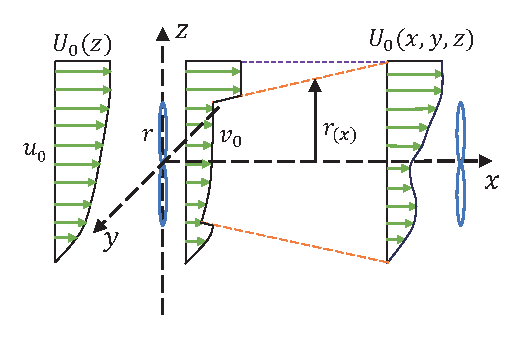
\includegraphics[width=\linewidth]{wakemodel.eps}
    \caption{A schematic diagram illustrating the 3D wind turbine wake effect.}
    \label{wakemodel}
    \end{figure}
    
    We can use the following wind shear model \cite{kim2012simulation} to simulate:
    \begin{equation}\label{E5}
    	U_0(z)=u_r\left(\frac{z}{z_r}\right)^\beta
    \end{equation}
    where $\beta$ represents the wind shear exponent, determined by real-world conditions. $u_r$ denotes the measured wind speed at the reference height $z_r$.
    
    \textcolor{blue}{To calculate the total flow in a circular cross-section in any wake region, it is necessary to determine the radius of initial generated wake $r_{(x)}$ at the horizontal axis $x$ and the average wind speed $v_0$ behind the blades of the turbine, which are defined as \cite{sun2018study}:}
   	\begin{equation}\label{E6}
   		\left\{
   		\begin{array}{c}
    	r_{(x)} = r + I \times x \\
    	v_0 = (1 - 2a) u_r
    	\end{array}
        \right.
    \end{equation}
    where $I$ denotes the wake decay constant, suggested as 0.05 for offshore wind farm; $a$ represents the factor which reflects the degree to which the wind flow is captured by the wind turbine rotor. The total flow rate $Q(x)$ consists of the flow $\pi r^2 v_0$ in the region of the rotor radius and the circulation in the circular region with radius $r$:
    \begin{equation}\label{E7}
    	Q(x) = \pi r^2 v_0 + \iint U_0(z) ds = \iint U_0(x,y,z) ds
    \end{equation}
    
    \textcolor{blue}{The model is based on the important assumption that the downwind wake exhibits a Gaussian distribution where the wind speed distribution at any height $z$ in the horizontal direction at the downwind position is as follows \cite{sun2023wind}:}
    \begin{equation}\label{E8}
    	U_0(x, y, z) = \frac{G(x)}{2\pi \eta^2} e^{-\frac{y^2 + (z - h)^2}{2 \eta^2}} + W(x) + U_0(z)
    \end{equation}
    where $G(x)$, $W(x)$, and $\eta$ are three parameters that need to be derived by derivation, which determine the shape of the Gaussian distribution. $\eta$ is defined as $\eta = \frac{r_x}{\xi}$, which aims to simplify the calculation. $\xi$ is an empirical parameter that is affected by a variety of factors such as incoming wind speed, turbulence intensity, and engineering reality. In this research, the recommended value is 1.98 \cite{tao2020wind}.
    
    Another assumption is that the wind speed is continuous at the wake boundary, implying that it can be expressed by \cite{tao2020wind}: 
    \begin{equation}\label{E9}
    	\left\{
    	\begin{array}{c}
    		\frac{G(x)}{2\pi \eta^2} e^{-\frac{y^2 + (z - h)^2}{2 \eta^2}} + W(x) + U_0(z) = U_0(z) \\
    		y^2 + (z - h)^2 = r_{(x)}^2
    	\end{array}
    	\right.
    \end{equation}
    
    After deriving the above few equations, $G(x)$ and $W(x)$ are expressed as follows \cite{sun2023wind}:
    \begin{equation}\label{E10}
    	 \left\{
    	\begin{array}{c}
        G(x) = \frac{Q(x) - \int \Delta U \, dz}{( 1 - e^{-\frac{\xi^2}{2}} - \frac{\xi^2}{2} e^{-\frac{\xi^2}{2}})} \\
    	W(x) = - \frac{G(x) \xi^2}{2 \pi r_{(x)}^2} e^{-\frac{\xi^2}{2}}   	
     	\end{array}
    	\right.
    \end{equation}
     where $\Delta U$ refers to the simplified wake speed after correcting for wind losses, which can be calculated by (\ref{E6}) to (\ref{E9}).
\section{Power-Law Perturbation-based Genetic Algorithm}
\label{sec_PPGA}
This section introduces the motivation of evolutionary adaption degree indicator and power-law perturbation in detail. Then the operating mechanism of PPGA is presented and the pseudo-code and illustrative diagram are given.
\subsection{Evolutionary Adaption Degree}
In GAs, genetic operations such as crossover and mutation help to recombine and generate new discrete solutions, thereby exploring new regions of the search space. These operations involve two critical stages: exploration and exploitation. Exploration refers to searching unvisited areas of the search space to discover potential optimal regions. Exploitation involves fine-tuning the search within already identified promising areas to improve the quality of solutions. Balancing these two stages is crucial for effective optimization \cite{10010703}. However, maintaining this balance is particularly challenging in complex discrete search spaces. This challenge has inspired us to develop an indicator that can assess the current robustness of the population and determine whether it can escape local optima and continue evolving towards the desired optimal solution. To this end, we use three characteristics that best reflect population quality: the diversity $D$, the proportion of stagnant individuals $S$, and solution quality $F\left(\varphi_i^t\right)$, to reflect this indicator. The evolutionary adaption degree can be expressed by:
\begin{equation}\label{E11}
	\theta= F\left(\varphi_i^t\right) \times \sqrt{Div}- S 
\end{equation}
where $\sqrt{Div}$ can reduce the impact of diversity on the evolution scale while smoothing fluctuations; $\varphi_i^t$ denotes independent population individual. The diversity of population is defined as: 
\begin{equation}\label{E12}
	Div = \frac{\sum_{i=1}^{N-1} \sum_{j=i+1}^{N} d_{ij}}{D_s \cdot (N \cdot (N - 1))}
\end{equation}
 where $D_s$ is the dimension of each individual and $N$ is the population size. $d_{ij}$ is the distance for each pair of individuals $i$ and $j$ in the population. Better solutions in a more diverse population can achieve higher scores. When the proportion of stagnant individuals $S$ is high, the negative impact becomes more significant, reducing the evolution scale $\theta$, signaling the need to break the stagnation. By measuring this evolutionary adaptation degree, we hope to explore the internal variation patterns of the population and assist the algorithm in overcoming evolutionary stagnation.
\subsection{Power-Law Perturbation}
Simultaneously, determining the extent of intervention for the population and how to implement reasonable and scientific perturbations is also an issue to be resolved. \textcolor{blue}{In nature, collective behaviors like fish schools or bird flocks exhibit scale-free patterns, where similar structures emerge across different scales, revealing underlying organization beyond individual actions.} Scholars have discovered stable and universal patterns from these natural phenomena — the power-law distribution. It can be calculated as:
\begin{equation}\label{E13}
	\sigma(x) = \varpropto x^{-\varepsilon},
\end{equation}
where $\sigma(x)$ is the probability density function of the variable. $\varpropto$ is the normalization constant. $\varepsilon$ is the exponent of the power-law distribution. \textcolor{blue}{Introducing the power-law distribution into the disturbance strategy of genetic algorithms aims to leverage its self-similarity and scale-free properties to aid the population in effective exploration and exploitation.}

Therefore, we propose a perturbation method based on the power-law distribution, utilizing its self-similarity and scale-free properties to help the population escape local optima and explore a wider range of the search space, continuously improving the quality of solutions. This method not only draws from universal natural principles but also demonstrates excellent performance in complex multimodal optimization problems \cite{zhou2020power}, i.e.,
\begin{equation}\label{E14}
\varphi_i^{t}=	\sigma\left(\varphi_i^{t}, 2.5\right)
	\end{equation}
where $\sigma\left(\varphi_i^{t}, 2.5\right)$ represents applying a power-law perturbation with an exponent of 2.5 to population. In many practical situations, the power-law exponent for various natural phenomena is close to 2.5. 
\subsection{PPGA Scheme}
In the initialization phase of the genetic algorithm, the first step is to generate an initial population $\Psi^t= \{\varphi^{t}_1,\varphi^{t}_2, ..., \varphi^{t}_n \}_{t=1}$. Each individual $\varphi_i^{t}$ in the population represents a potential solution, and in the wind farm problem, each individual represents a potential turbine layout. During this phase, it is necessary to convert the turbine position encoding into three-dimensional coordinates and generate the initial solution space for the wind farm. Assuming the turbine position is encoded as $(i,j)$, it can be converted to actual three-dimensional coordinates $(x,y,z)$ using the following matrix formula:
\begin{equation}\label{E15}
\begin{bmatrix}
	x \\
	y \\
	z
\end{bmatrix}
=
\begin{bmatrix}
	s_x &  &  \\
	 & s_y & \\
	 &  & h
\end{bmatrix}
\begin{bmatrix}
	i \\
	j \\
	1
\end{bmatrix}
\end{equation}
where $s_x$ is the spacing of the grid in the $x$ direction; $s_y$ is the spacing of the grid in the $y$ direction; $h$ is the fixed height of the turbine. The wind farm area is divided into discrete grids, and turbine positions are encoded as discrete integer values. For each individual $\varphi_i^{t}$, the discrete encoding is represented by these values. Using a three-dimensional matrix, each turbine's grid point is converted into its actual three-dimensional coordinates. All generated turbine layouts are then combined to form the initial population.

Then, the crossover operation is a crucial mechanism for producing new individuals, aimed at combining the traits of parent individuals to form new offspring. The feature mapping crossover combines the advantages of standard crossover by mapping and mixing features from parent individuals to generate new ones. It not only considers various aspects of the parent individuals but also utilizes the relationships between features for more complex combinations, thus enhancing the exploration capabilities of the search space. The process of generating new individuals is described by the following formula:
\begin{equation}\label{E16}
	\varphi_i^{\text {new }}=C_r \times \varphi^t_i[:]+ (1-C_r) \times \varphi^t_j[:]
\end{equation}
where $C_r$ is the crossover rate vector, while $\varphi^t_i[:]$ and $\varphi^t_j[:]$ represent the feature vectors of the two parent individuals. This operation allows the algorithm to generate more diverse individuals, thereby improving the exploration capability of the algorithm.

The mutation operation introduces a new excitation mechanism, effectively preventing the population from prematurely converging to a local optimum. It helps the algorithm to perform a broader search in the solution space, discovering new potential solutions. Based on the set mutation rate, each individual in the population is checked to decide whether to apply the mutation operation. This process can be represented by:
\begin{equation}\label{E17}
%	\varphi^t_i[:]= 	\varphi_i^t , \quad \text{if} \ rand < p_m  
	\varphi^{new}_i[j] = rand \times (\varphi^{up}_i-\varphi^{low}_i) \quad \text{if} \ rand < p_m  
\end{equation}
where $j$ denotes the dimension index of individual $\varphi^{new}_i$; $\varphi^{up}_i$ and $\varphi^{low}_i$ mean individuals' upper and lower boundaries, respectively. $rand$ is a random value distributed over the range [0, 1). The mutation rate $p_m$ determines the likelihood of each gene undergoing mutation. $p_m$ is set as 0.1 as recommended in this study.

After mutation, fitness evaluation is a crucial step in determining the performance of each individual during the evolutionary process. The population is sorted in descending order based on the fitness $F\left(\varphi_i^t\right)$ of each individual. The top $k$ individuals with the highest fitness are selected as the elite individuals, which will proceed to the next generation.

Starting from the second generation, before the new population enters the next evolutionary cycle, we aim to assess the overall quality of the current generation. \textcolor{blue}{By using (\ref{E11}), we obtain the evolutionary adaptation degree $\theta$, which serves as a quantitative metric to gauge the population’s state from multiple dimensions. This indicator provides an intuitive understanding of the population’s quality, diversity, and evolutionary vitality. Based on this evaluation, the intervention decisions are made: 1) When the population's indicators are all favorable, we deem it unnecessary to interfere with the population. This avoids disrupting promising evolutionary trajectories, minimizes counterproductive effects, and reduces computational costs \cite{JAS-2024-0370}. 2) When evolutionary adaptation degree $\theta$ falls below a critical threshold, we consider intervening in the population by adding power-law perturbations to some individuals. A low $\theta$ value indicates potential issues, such as the population becoming trapped in a local optimum, a significant reduction in diversity, or stagnation in evolutionary progress. In such cases, we consider applying power-law perturbations to selectively intervene in the population. A perturbation value is applied to each dimension of an individual, meaning the generated perturbation is added to adjust its position in the search space. These perturbations aim to reintroduce variability and vitality by adjusting the positions or genetic structures of certain individuals.} Therefore, the value $\theta$ not only effectively describes the tail behavior of the data but also maintains the stability of the distribution. This process can be represented by:
\begin{equation}\label{E18}
	\varphi_i^{t+1}= \begin{cases}\sigma\left(\varphi_i^{t}, 2.5\right), & \text{if}\; rand<\theta'- \theta_i \;\&\; \theta_i<\theta' \\ \varphi_i^{t}, & \text {otherwise}\end{cases}
\end{equation}
where $\theta'$ and $\theta_i$ denotes the threshold value and current iteration value of evolutionary adaptation degree, respectively. $rand$ is distributed random in [0, 1). 

\textcolor{blue}{The scale-free nature of the power-law distribution inherently balances the magnitude and frequency of perturbations. This dual capability supports efficient exploitation of high-potential areas while continuing to explore alternative paths to the global optimum. By escaping local optima and maintaining the structured diversity of the population, power-law perturbations can prevent the commonly premature convergence issue.} When considering the time to perturb and the measure of perturbation for solutions that have lost vitality and become trapped in local optima, we find that the probability of perturbation is strongly correlated with the positive and negative feedback occurring within the population. Subsequent ablation experiments also confirm our hypothesis that appropriate interference with the population significantly enhances its overall performance. Therefore, the probability of the occurrence of $rand$ is a means of regulating power-law perturbations.
\begin{figure}[!t]
	\centering
	%\setlength{\abovecaptionskip}{-0.2cm}
	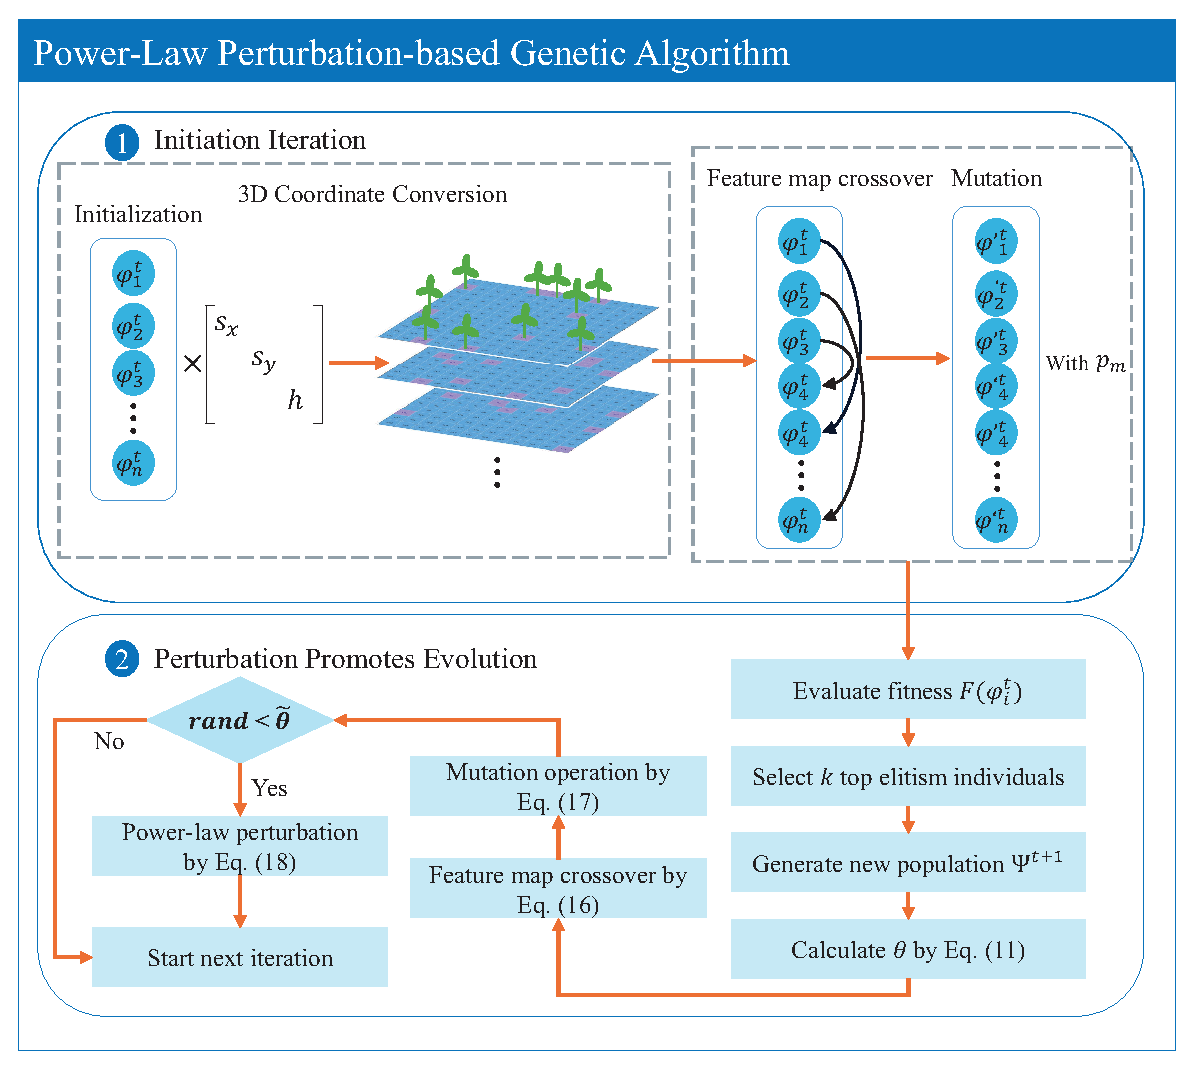
\includegraphics[width=\linewidth,scale=1]{PPGA.eps}
	\caption{The flowchart of PPGA.}
	\label{ppga}
\end{figure}

The general process of PPGA is illustrated by Fig.~\ref{ppga}. Algorithm \ref{alg1} reveals the pseudo-code of PPGA. In the first iteration, the population follows the classic genetic algorithm process of initialization, crossover, mutation, evaluation, and selection. Starting from the second generation, the evolutionary adaptation degree is calculated according to (\ref{E11}) to determine whether the population needs stimulation. After the mutation phase, a power-law perturbation is applied to the entire population based on the evolutionary adaption degree $\theta$ by~(\ref{E18}), driving the population towards a power-law distribution. Subsequently, elite individuals are selected to enter the next round of evolution.

\subsection{\textcolor{blue}{Computational complexity analysis}}
\textcolor{blue}{Computational complexity analysis helps evaluate the efficiency of the algorithm in practical applications, especially when the problem scale increases, as optimizing execution time and resource consumption becomes crucial.}

\textcolor{blue}{The computational complexity primarily depends on the population size $N$ and the problem dimension $D$. For PPGA, the fitness evaluation process has a complexity of $O(N \cdot D)$ for each generation. The selection step, which involves sorting the population, has a computational complexity of $O(N \cdot logN)$. The complexity of evolutionary adaption degree can be calculated as $O(N^2 \cdot D)$ due to the need to create a diversity matrix. The power-law perturbation function costs $O(N \cdot D)$. The complexities of other operations are relatively small and can generally be ignored. Therefore, the overall computational complexity of PPGA is $O(N^2 \cdot D + 2N \cdot D + N \cdot logN)$.}

\textcolor{blue}{The computational complexity of basic genetic algorithm is $O(N \cdot D + N \cdot logN)$. Although the computational complexity has increased, the required population size for this problem is relatively small, making the additional computational resources acceptable compared to the performance improvement.}	
\subsection{Advantages and novelty}
The advantages and novelty of this work can be summarized as follows:
\begin{itemize}
	\item [1)]We originally propose an indicator called evolutionary adaptation degree, which focuses on the core factors of the population by integrating diversity, stagnation proportion, and solution quality. 
	\item [2)]We introduce a power-law perturbation mechanism into the genetic algorithm to incorporate controlled randomness, enabling the algorithm to escape local optima, maintain population diversity.
	\item [3)]For 3D wind farm layout optimization problem, we assess population vitality in real time and apply power-law perturbation when needed to enhance adaptive exploration of complex solution spaces.
\end{itemize}

\begin{algorithm}[!t]
	\caption{The pseudo-code of PPGA}
	\DontPrintSemicolon
	\label{alg1} 
	\tcc{Initialization Population  $\Psi_0$} 	
	\For{$t=1$ \KwTo $iter_{MAX}$}{		
		\tcc{Crossover}
		\For{$i = 1$ \KwTo $N$}
		{
			Randomly select two parents $\varphi_q$ and $\varphi_j$. \;
			Feature mapping crossover new offspring by (\ref{E16}). \;
		}
		
		\tcc{Mutation}
		\For{$i = 1$ \KwTo $N$}{
			Mutating individuals by (\ref{E17}). \;		
		}
		\tcc{Power-Law Perturbation}
			\If{$ t\geq2 \;\&\; rand<\theta'- \theta_i \;\&\; \theta_i<\theta'$}
			{
				Apply power-law perturbation by (\ref{E18}). \;
			}		
		\tcc{Evaluation and Elitism Selection}
		Evaluate the fitness of all individuals in the new population. \;
        Retain the best individuals to update the new population $\Psi^{t+1}$. \;
        
        \tcc{Judge evolutionary status}
		Calculate evolutionary adaptation degree $\theta$ for $\Psi^{t+1}$. \;
		
	}
\end{algorithm}


\section{Experiments and Analysis}
\label{sec_experiment}
To validate the performance of PPGA within the 3D wind farm optimization framework, we select the terrain of an actual wind farm as a case study. We compare PPGA with other state-of-the-art algorithms under different complex wind conditions. \textcolor{blue}{RLPS-TLBO \cite{ling2024multi}, SUGGA \cite{sugga}, AGA \cite{aga}, CGPSO \cite{lei2023chaotic}, and MDPSO \cite{tao2020wind} are currently the most advanced algorithms for this problem. SHADE \cite{tanabe2013success}, INFO \cite{ahmadianfar2022info}, FBIO \cite{chou2020fbi}, and FLA \cite{hashim2023fick} are representative and novel swarm intelligence algorithms. DE \cite{storn1997differential} and PSO \cite{kennedy1995particle} are classical evolutionary algorithms applied for practical  problems.} Data analysis and visualization, determination of optimal parameters, and discussions on optimization deceleration are implemented to comprehensively analyze the algorithm and framework. 
\subsection{Experimental Setup}
In this study, we employ the H171-6.2MW model wind turbine of China Haizhuang company. The specific parameters of the wind turbine are shown in Table \ref{turbine}. Because the sea surface is flat and free of obstacles, this study does not consider obstacle constraints. We take Nantong Offshore Wind Farm H1, the largest single offshore wind project in China, as an example. The project site is rectangular in shape, with a length of about 8 km from north to south and a width of about 5 km from east to west, with a planned site area of about 40 $\text{km}^2$ and a planned installed capacity of 250 MW. The seabed topography is relatively gentle, and the depth of the water ranges from 6 to 13 m. To match the actual conditions, we select four wind scenarios in 2023. The wind data is sourced from the offshore monitoring stations of this project. Fig.~\ref{windrose} shows the distribution and intensity of these four wind conditions. This set of wind condition data includes 16 directions and 7 different wind speed distributions.

This experimental conditions are Windows 11 with AMD Ryzen 7 5700X 8-Core Processor CPU 3.40 GHz. The runtime of independent control experiments is set to 30 epochs. The number of optimization iteration is defined as 50. All parameters about algorithms are listed in Table \ref{parameters}.
\begin{figure}[!t]
	\centering
	%\setlength{\abovecaptionskip}{-0.2cm}
	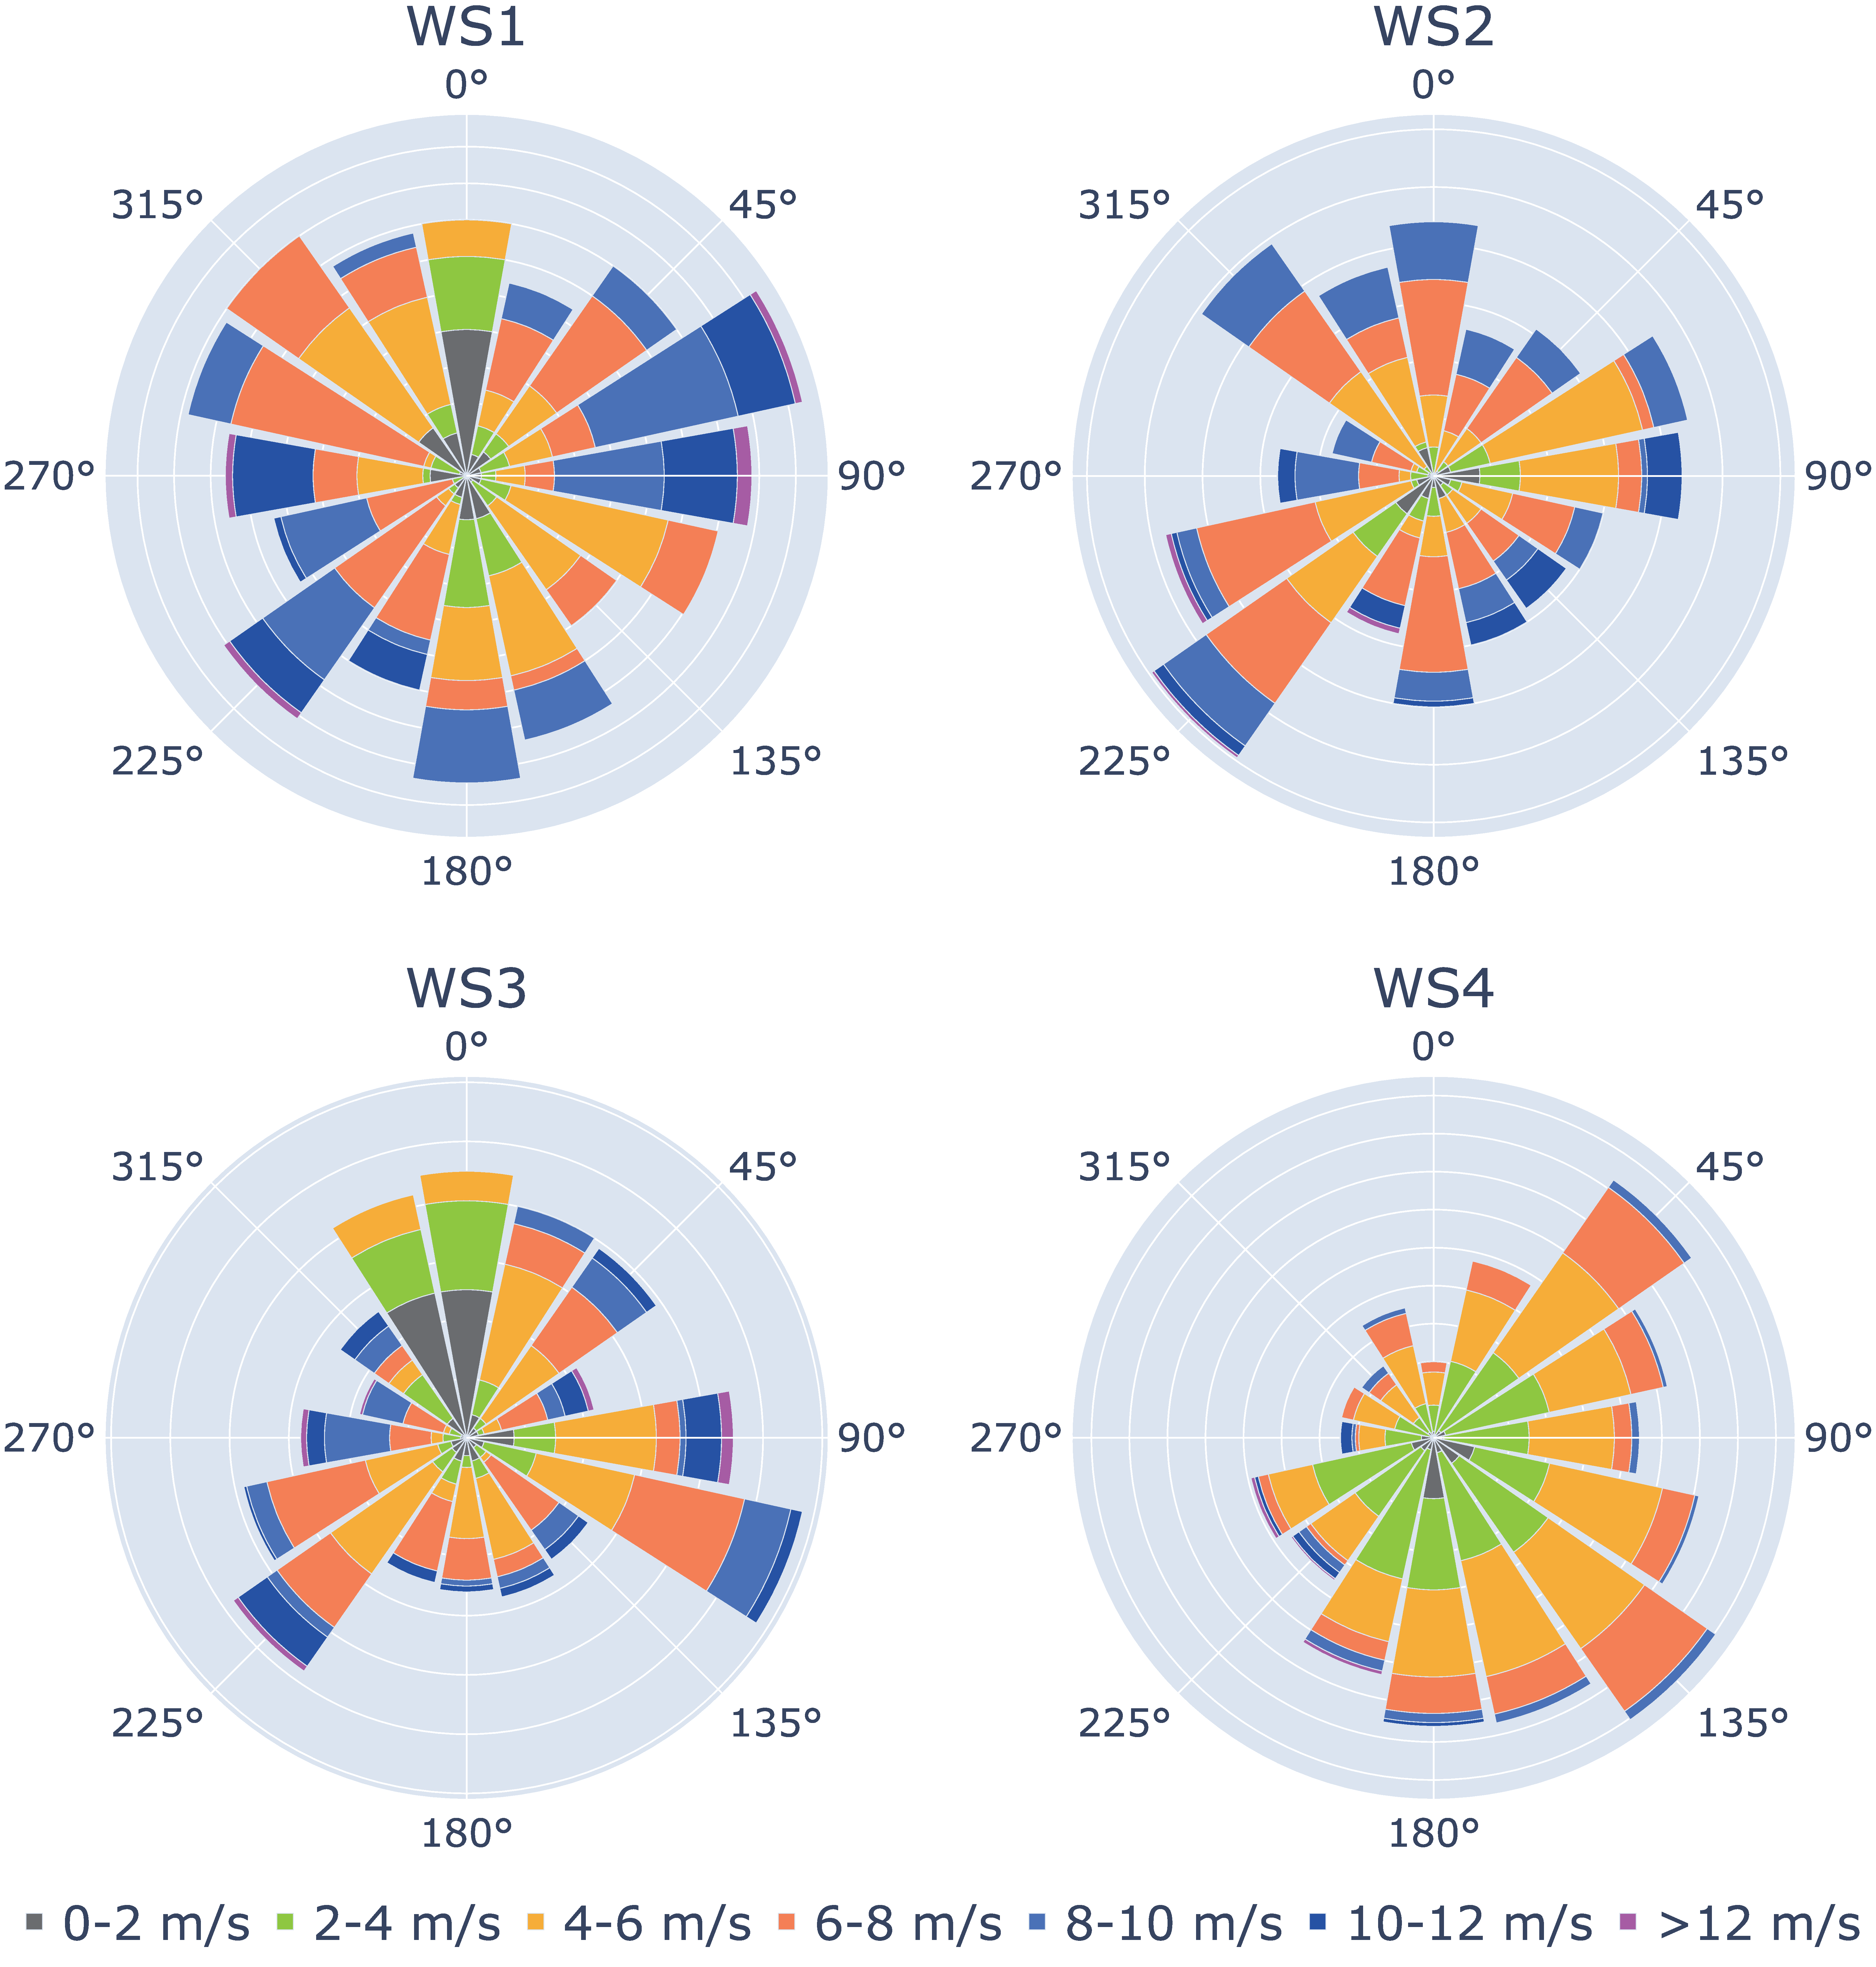
\includegraphics[width=.98\linewidth]{windrose.eps}
	\caption{Four wind scenario roses.}
	\label{windrose}
\end{figure}

\begin{table}[t!]
	\centering
	\caption{Typical setup related to wind turbines and farms.}
	\begin{tabular}{llll}
		\hline
		Rotor diameter   & 171 m  &  Hub height  & 107 m \\ 
		Rated voltage   & 690 v   &  Rated power  & 6200 kw  \\ 
		Turbine spacing    & 300 m  & Farm size &  5 km $\times$ 8 km \\ \hline
	\end{tabular}\label{turbine}
\end{table}


\begin{table}[t!]\color{blue}
	\centering
	\caption{Parameter settings of the experimental group.}
	\label{parameters}
	\begin{tabular}{lcl}
		\hline
		Algorithm          & Year & Settings \\
		\hline
		PPGA    &  ---   & $N_i=30, \theta'=0, C_r=0.8, p_m=0.1$ \\
		RLPS-TLBO & 2024 & $N_i=30, n_t = 4 $ \\
		CGPSO & 2023   & $N_i=30, p_m = 0.01, c = 1.49618$   \\
		FLA     & 2023   &   $N_i=30, c_1=0.1, c_2=0.2$ \\
		INFO     & 2022    & $N_i=30, p_r=0.03$  \\
		MDPSO  & 2020 & $N_i=30, p_m = 0.01$ \\
		FBIO  & 2020 & $N_i=30, p_r=0.03$ \\
		SUGGA  & 2019 &  $N_i=30, C_r=0.8, p_m=0.1$ \\
		AGA  & 2019 &  $N_i=30, C_r=0.8, p_m=0.1$\\
		SHADE  & 2013 &  $N_i=30, M_F=0.5, C_r=0.5$ \\
		DE  & 1997 & $N_i=30, M_F=0.5, C_r=0.5$ \\
		PSO  & 1995 & $N_i=30, p_m = 0.01$ \\ \hline
	\end{tabular}
\end{table}
\subsection{Results in Different Wind Conditions }\label{turbines}
We use the Wilcoxon rank-sum test to evaluate the performance of different algorithms. This statistical method is robust to outliers, providing more reliable results. It is suitable for comparing two independent samples and can effectively assess the performance differences between two algorithms on the same problem \cite{7113903,10460144}. Under four complex wind conditions, we attempt to place 20, 30, 40, and 50 turbines in the wind farm. In practical engineering, the number of turbines generally ranges between 20 and 40. When the number of turbines is too high, the combined wake effects and the exponentially increasing cost and time of computation become significant factors.
\begin{table*}[ht!]\color{blue}
	\centering
	\caption{The optimal $E$ for different numbers of wind turbines at wind condition WS1.}
	\label{WS1}
	\renewcommand\arraystretch{1}
	\setlength\tabcolsep{5pt}{
		\begin{tabular}{lllll} \cline{1-5}
			Algorithm & 20 Num. & 30 Num. & 40 Num. & 50 Num. \\	\cline{1-5}	
			PPGA	 &	\textbf{85.64(4.79E-04)}	 &	\textbf{74.20(2.07E-04)}	 &	\textbf{67.72(7.94E-05)}	 &	\textbf{63.47(6.85E-05)}	\\
			RLPS-TLBO & 77.83(1.13E-04)+    &  66.16(2.04E-05)+   &   59.64(1.66E-05)+ & 54.81(6.58E-06)+ \\
			CGPSO	 &	79.90(1.18E-04)+	 &	67.69(5.45E-05)+	 &	60.68(2.79E-05)+	 &	55.92(3.23E-05)+	\\
			FLA	     &	79.28(1.94E-04)+	 &	67.41(1.17E-04)+	 &	60.04(4.85E-05)+     &	55.62(3.51E-05)+   \\
			INFO	 &	79.76(6.54E-04)+	 &	67.73(1 32E-04)+	 &	60.49(7.15E-05)+     &	55.72(5.47E-05)+	\\
		    MDPSO    &  80.42(4.16E-04)+    &  68.70(1.51E-04)+   &   61.49(6.50E-05)+ & 56.62(5.52E-05)+  \\
		    FBIO	 &	81.56(1.80E-04)+	 &	68.89(9.16E-05)+	 &	61.38(3.03E-05)+     &	56.23(1.80E-05)+    \\
			SUGGA	 &	83.46(3.43E-04)+	 &	71.48(1.51E-04)+	 &	64.73(8.88E-05)+	 &	60.06(5.85E-05)+    \\
			AGA	     &	84.36(4.21E-04)+	 &	73.10(1.40E-04)+	 &	66.65(5.56E-05)+	 &	61.72(3.70E-05)+	\\
			SHADE	 &	78.38(6.15E-05)+	 &	66.69(5.41E-05)+	 &	59.60(2.38E-05)+	 &	54.77(3.12E-05)+	\\
			 DE	     &	77.99(7.11E-05)+	 &	66.27(5.45E-05)+	 &	59.35(1.40E-05)+	 &	54.56(1.58E-05)+	\\
			 PSO	 &	79.37(9.55E-05)+	 &	67.38(5.70E-05)+	 &	60.42(1.52E-05)+	 &	55.82(2.06E-05)+	\\	 \cline{1-5}
			$w/t/l$  &	11/0/0	 &	11/0/0	 &	11/0/0	 &	11/0/0	\\ \cline{1-5}
	\end{tabular}}
\end{table*}

\begin{table*}[ht!]\color{blue}
	\centering
	\caption{The optimal $E$ for different numbers of wind turbines at wind condition WS2.}
	\label{WS2}
	\renewcommand\arraystretch{1}
	\setlength\tabcolsep{5pt}{
		\begin{tabular}{lllll} \cline{1-5}
			Algorithm & 20 Num. & 30 Num. & 40 Num. & 50 Num. \\	\cline{1-5}
			PPGA	 &	\textbf{85.53(2.76E-04)}	 &	\textbf{74.19(1.48E-04)}	 &	\textbf{67.77(9.05E-05)}		 &	\textbf{63.37(6.68E-05)}	\\
			RLPS-TLBO & 77.72(4.58E-05)+    &  66.30(3.47E-05)+   &   59.48(1.77E-05)+ & 54.83(1.30E-05)+ \\
			CGPSO	 &	79.53(1.15E-04)+	 &	67.99(3.79E-05)+	 &	60.75(2.81E-05)+         &	55.88(1.73E-05)+    \\
			FLA	     &	79.30(3.39E-04)+	 &	67.28(1.35E-04)+	 &	60.19(5.80E-05)+		 &	55.28(3.79E-05)+ \\		
			INFO	 &	79.46(4.55E-04)+	 &	67.38(8.09E-05)+	 &	60.50(1.03E-04)+		 &	55.54(4.81E-05)+	\\
			MDPSO    &  80.16(4.55E-04)+     &  68.46(1.94E-04)+     &   61.30(7.87E-05)+        &   56.72(8.32E-05)+  \\
			FBIO	 &	81.55(1.19E-04)+	 &	68.91(3.84E-05)+	 &	61.50(3.39E-05)+	     &	56.40(1.77E-05)+	\\
			SUGGA	 &	83.61(4.94E-04)+	 &	71.55(1.38E-04)+	 &	64.97(5.79E-05)+		 &	60.08(5.49E-05)+	\\
			AGA	     &	84.86(2.93E-04)$\approx$	 &	73.36(1.99E-04)+	 &	66.80(5.20E-05)+		 &	61.77(4.16E-05)+	\\	
			SHADE	 &	78.30(8.16E-05)+	 &	66.66(4.80E-05)+	 &	59.65(3.36E-05)+		 &	54.82(1.71E-05)+ \\
			DE	     &	77.93(5.25E-05)+	 &	66.49(4.15E-05)+	 &	59.34(1.63E-05)+	 &	54.71(1.24E-05)+	\\
			PSO	 &	79.03(6.09E-05)+	 &	67.71(2.76E-05)+	 &	60.56(2.15E-05)+	 &	55.73(1.24E-05)+	\\   \cline{1-5}
			$w/t/l$  &	10/1/0	 &	11/0/0	 &	11/0/0	 &	11/0/0	\\ \cline{1-5}
	\end{tabular}}
\end{table*}

\begin{table*}[ht!]\color{blue}
	\centering
	\caption{The optimal $E$ for different numbers of wind turbines at wind condition WS3.}
	\label{WS3}
	\renewcommand\arraystretch{1}
	\setlength\tabcolsep{5pt}{
		\begin{tabular}{lllll} \cline{1-5}
			Algorithm & 20 Num. & 30 Num. & 40 Num. & 50 Num. \\	\cline{1-5}
			PPGA	 &	\textbf{90.31(9.89E-04)}	 & \textbf{79.51(4.96E-04)}	 &	\textbf{72.31(1.25E-04)}	 &	\textbf{66.10(1.25E-04)}	\\
			RLPS-TLBO & 79.11(6.99E-05)+    &  68.08(3.82E-05)+   &   61.22(1.94E-05)+ & 56.46(1.31E-05)+ \\
			CGPSO	 &	81.08(1.18E-04)+	 & 69.75(8.95E-05)+	 &	62.53(4.37E-05)+	 &	57.52(4.14E-05)+	\\
			FLA	     &	81.65(2.88E-04)+	 &	69.80(9.70E-05)+ &	62.68(9.51E-05)+	 &	57.51(7.33E-05)+	\\
			INFO	 &	81.93(4.46E-04)+	 &	70.08(1.88E-04)+ &	62.88(1.42E-04)+	 &	57.55(7.25E-05)+	\\
			MDPSO    &  81.52(4.88E-04)+     &  70.42(1.53E-04)+     &   62.99(1.83E-04)+        &   58.41(1.15E-04)+  \\
			FBIO	 &	84.94(1.12E-04)+	 &	71.91(4.42E-05)+ &	64.37(3.55E-05)+	 &	58.74(2.35E-05)+	\\
			SUGGA	 &	86.01(2.65E-04)+	 & 75.30(1.47E-04)+	 &	68.16(1.18E-04)+	 &	62.47(9.59E-05)+	\\
			AGA	     &	88.50(3.31E-04)+	 & 77.65(2.55E-04)+	 &	69.75(9.14E-05)+	 &	64.18(5.62E-05)+	\\
			SHADE	 &	81.55(8.43E-05)+	 & 69.68(3.38E-05)+	 &	62.47(3.88E-05)+	 &	57.28(2.14E-05)+ \\	
			DE	     &	80.90(3.51E-05)+	 &	69.34(2.01E-05)+	 &	62.26(5.87E-05)+	 &	57.13(1.52E-05)+	\\
			PSO	 &	80.89(6.49E-05)+	 &	69.22(4.99E-05)+	 &	62.30(2.59E-05)+	 &	57.26(1.27E-05)+	\\					
			 \cline{1-5}
			$w/t/l$  &	11/0/0	 &	11/0/0	 &	11/0/0	 &	11/0/0	\\ \cline{1-5}
	\end{tabular}}
\end{table*}

\begin{table*}[ht!]\color{blue}
	\centering
	\caption{The optimal $E$ for different numbers of wind turbines at wind condition WS4.}
	\label{WS4}
	\renewcommand\arraystretch{1}
	\setlength\tabcolsep{5pt}{
		\begin{tabular}{lllll} \cline{1-5}
			Algorithm & 20 Num. & 30 Num. & 40 Num. & 50 Num. \\	\cline{1-5}	
			PPGA	 &	\textbf{92.62(4.32E-04)}	 &	\textbf{81.45(3.35E-04)}	 &	\textbf{74.28(1.80E-04)}	 &	\textbf{68.99(8.29E-05)}	\\
			RLPS-TLBO & 87.09(1.88E-04)+    &  72.55(1.56E-04)+   &   63.56(1.34E-05)+ & 58.63(1.13E-05)+ \\
			CGPSO	 &	83.96(1.23E-04)+	 &	72.36(4.80E-05)+	 &	64.46(2.39E-05)+	 &	59.34(2.92E-05)+	\\
			FLA	     &	84.48(1.80E-04)+	 &	72.07(9.61E-05)+	 &	64.56(5.09E-05)+	 &	59.59(4.71E-05)+	\\
			INFO	 &	85.32(3.17E-04)+	 &	73.49(3.88E-04)+	 &	65.39(1.40E-04)+	 &	59.78(1.35E-04)+	\\
			MDPSO    &  85.86(2.73E-04)+     &  72.63(1.75E-04)+     &   65.16(6.37E-05)+        &   60.06(5.36E-05)+  \\
			FBIO	 &	88.90(2.08E-04)+	 &	74.96(5.61E-05)+	 &  66.06(2.60E-05)+	 &	60.55(2.01E-05)+	\\
			SUGGA	 &	87.35(1.63E-04)+	 &	75.52(1.23E-04)+	 &	68.20(1.03E-04)+	 &	63.54(3.59E-05)+	\\
			AGA	     &	91.25(4.08E-04)+	 &	79.67(1.19E-04)+	 &	72.04(7.59E-05)+	 &	66.58(4.75E-05)+	\\
			SHADE	 &	84.65(7.64E-05)+	 &	72.36(8.52E-05)+	 &	64.46(2.90E-05)+	 &	59.01(1.21E-05)+	\\
			DE	     &	84.10(4.92E-05)+	 &	71.89(7.03E-05)+	 &	64.18(2.01E-05)+	 &	58.80(5.86E-06)+	\\
			PSO	 &	83.71(5.32E-05)+	 &	72.12(2.42E-05)+	 &	64.27(8.51E-06)+	 &	59.09(1.36E-05)+	\\			
			 \cline{1-5}
			$w/t/l$  &	11/0/0	 &	11/0/0	 &	11/0/0	 &	11/0/0	\\ \cline{1-5}
	\end{tabular}}
\end{table*}

\begin{table*}[htbp!] \color{blue}
	\centering
	\caption{The detailed $p$-values for Wilcoxon rank-sum test of 16 conditions.}
	\label{pvalue}
	\setlength\tabcolsep{2pt}{
		\begin{tabular}{cccccccccccc}
			\cline{1-12}
			PPGA vs	 &	RLPS-TLBO		&	CGPSO		 &	FLA		&	INFO		&	MDPSO		&	FBIO		&	SUGGA	& AGA & SHADE & DE & PSO	\\	\cline{1-12}
			WS1-20 Num.	 &	2.87E-11 +	 &	5.23E-11 +	 &	3.88E-11 +	 &	1.23E-11 +	 &	1.02E-11 +	 &	3.06E-11 +	&   2.46E-04 +	& 4.68E-02 + & 2.87E-11 +& 2.87E-11 +& 2.87E-11 +\\	
		    WS1-30 Num.	 &	2.87E-11 +	 &	2.87E-11 +	 &	2.87E-11 +	 &	2.87E-11 +	 &	2.87E-11 +	 &	2.87E-11 +	&   2.49E-11 + &  2.56E-03 + &	 2.87E-11 + & 2.87E-11 +& 2.87E-11 +\\	
			WS1-40 Num.	 &	2.87E-11 +	 &	2.87E-11 +	 &	2.87E-11 +	 &	2.87E-11 +	 &	2.87E-11 +	 &	2.87E-11 +	&   3.51E-11 + &  6.97E-06 + & 2.87E-11 +& 2.87E-11 +& 2.87E-11 +	\\	
			WS1-50 Num.	 &	2.87E-11 +	 &	2.87E-11 +	 &	2.87E-11 +	 &	2.87E-11 +	 &	2.87E-11 +	 &	2.87E-11 +	&	2.87E-11 + & 3.64E-10 + & 2.87E-11 +& 2.87E-11 +& 2.87E-11 +	\\	
			WS2-20 Num.	 &	2.87E-11 +	 &	2.87E-11 +	 &	4.28E-11 +	 &	7.76E-11 +	 &	6.37E-11 +	 &	1.27E-10 +	&	6.73E-04 + & 2.25E-01 $\approx$ & 2.87E-11 +& 2.87E-11 +& 2.87E-11 +	\\	
			WS2-30 Num.	 &	2.87E-11 +	 &	2.87E-11 +	 &	2.87E-11 +	 &	2.87E-11 +	 &	2.87E-11 +	 &	2.87E-11 +	&	1.94E-09 + & 4.10E-02 + & 2.87E-11 +& 2.87E-11 +& 2.87E-11 +	\\	
			WS2-40 Num.	 &	2.87E-11 +	 &	2.87E-11 +	 &	2.87E-11 +	 &	2.87E-11 +	 &	2.87E-11 +	 &	2.87E-11 +	&	6.37E-11 + & 3.96E-05 + & 2.87E-11 +& 2.87E-11 +& 2.87E-11 +	\\	
			WS2-50 Num.	 &	2.87E-11 +	 &	2.87E-11 +	 &	2.87E-11 +	 &	2.87E-11 +	 &	2.87E-11 +	 &	2.87E-11 +	&	2.87E-11 + & 3.66E-09 + & 2.87E-11 +& 2.87E-11 +& 2.87E-11 +	\\
			WS3-20 Num.	 &	2.87E-11 +	 &	2.87E-11 +	 &	3.88E-11 +	 &	7.76E-11 +	 &	5.77E-11 +	 &	1.77E-09 +	&	3.13E-07 + & 1.73E-02 + &	2.87E-11 +& 2.87E-11 +& 2.87E-11 + \\	
			WS3-30 Num.	 &	2.87E-11 +	 &	2.87E-11 +	 &	2.87E-11 +	 &	2.87E-11 +	 &	2.87E-11 +	 &	2.87E-11 +	&	2.13E-09 + & 7.91E-04 + &	2.87E-11 + & 2.87E-11 +& 2.87E-11 +\\	
			WS3-40 Num.	 &	2.87E-11 +	 &	2.87E-11 +	 &	2.87E-11 +	 &	2.87E-11 +	 &	2.87E-11 +	 &	2.87E-11 +	&	5.77E-11 + & 5.84E-10 + & 2.87E-11 +& 2.87E-11 +& 2.87E-11 +	\\	
			WS3-50 Num.	 &	2.87E-11 +	 &	2.87E-11 +	 &	2.87E-11 +	 &	2.87E-11 +	 &	2.87E-11 +	 &	2.87E-11 +	&	2.87E-11 + & 6.24E-09 + & 2.87E-11 +& 2.87E-11 +& 2.87E-11 +	\\	
			WS4-20 Num.	 &	1.15E-10 +	 &	2.87E-11 +	 &	2.87E-11 +	 &	3.88E-11 +	 &	3.51E-11 +	 &	1.93E-08 +	&	8.56E-11 + & 1.35E-02 + & 2.87E-11 + & 2.87E-11 +& 2.87E-11 +\\	
			WS4-30 Num.	 &	3.18E-11 +	 &	2.87E-11 +	 &	2.87E-11 +	 &	3.51E-11 +	 &	2.87E-11 +	 &	2.87E-11 +	&	3.51E-11 + & 1.81E-05 + & 2.87E-11 +& 2.87E-11 +& 2.87E-11 +	\\	
			WS4-40 Num.	 &	2.87E-11 +	 &	2.87E-11 +	 &	2.87E-11 +	 &	2.87E-11 +	 &	2.87E-11 +	 &	2.87E-11 +	&	2.87E-11 + & 4.89E-08 + & 2.87E-11 +& 2.87E-11 +& 2.87E-11 +	\\	
			WS4-50 Num.	 &	2.87E-11 +	 &	2.87E-11 +	 &	2.87E-11 +	 &	2.87E-11 +	 &	2.87E-11 +	 &	2.87E-11 +	&	2.87E-11 + & 1.69E-10 + & 2.87E-11 +& 2.87E-11 +& 2.87E-11 +	\\	 \cline{1-12}																			
	\end{tabular}}
\end{table*}
Tables \ref{WS1} $-$ \ref{WS4} show the optimal wind farm energy conversion efficiencies achieved by different algorithms under various experimental conditions. The numbers in parentheses represent the standard deviations of the data. $+$ indicates that PPGA outperforms the other algorithms in the statistical test. $w/t/l$ represent the win/tie/loss count of the target algorithm compared with others under each experimental condition. In all 16 scenarios, PPGA achieves the highest energy conversion efficiency, with the best values highlighted in bold. As the number of turbines increases, the complexity of wake effects also increases. Other algorithms' optimization capabilities decline rapidly, whereas PPGA continues to achieve optimal results, widening the performance gap with other algorithms. To further validate the potential of PPGA and ensure fairness, we have listed the $p$-value levels for all control groups in Table \ref{pvalue}. The $p$-value effectively avoids bias caused by factors such as sample size, data skewness, or outliers, ensuring that comparisons between different algorithms or experimental conditions are based on true differences rather than random factors. Under 16 experimental conditions, PPGA demonstrates statistically significant advantages with $p$-values below 0.05 compared to the other nine algorithms. PPGA only does not exhibit a significant difference from AGA in the WS2-20 Num. case. Because evolutionary fitness is evaluated in real-time, it endows the algorithm with the ability to continuously evolve. This also demonstrates that PPGA can maintain excellent performance when dealing with complex conditions. \textcolor{blue}{Notably, the experimental results demonstrate that GA-based algorithms surpass PSO-based and DE-based algorithms in both optimization performance and robustness, underscoring their unique advantages for this problem.}

\begin{figure*}[t!]\color{blue}
	\centering
	%\setlength{\abovecaptionskip}{-0.2cm}
	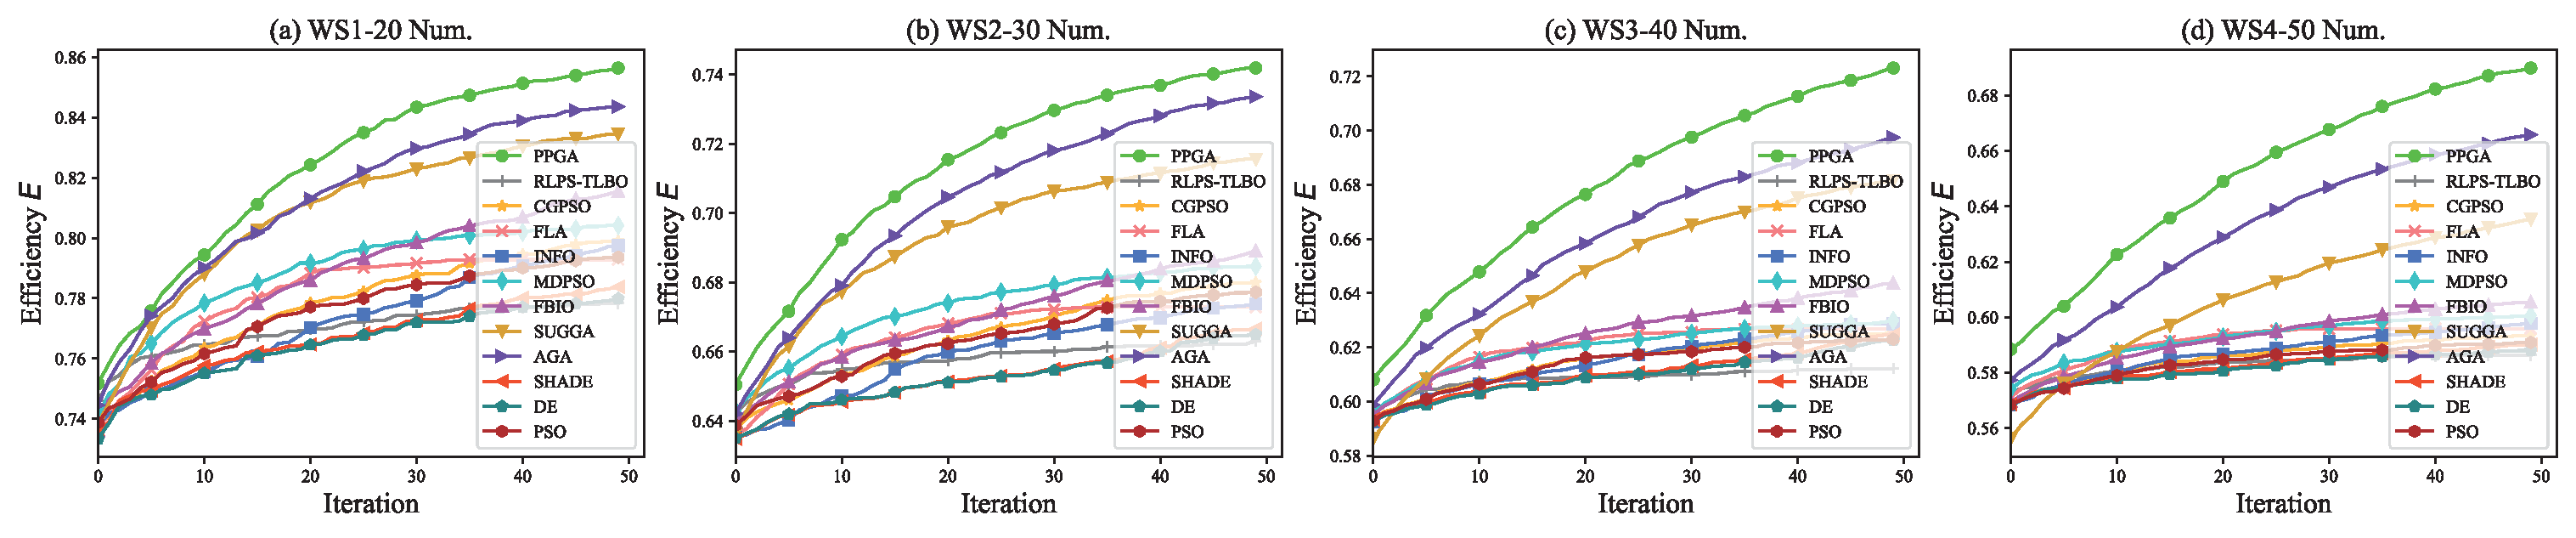
\includegraphics[width=\linewidth,scale=1.00]{conv.eps}
	\caption{Convergence trend charts of different algorithms under four representative experimental conditions.}
	\label{conv}
\end{figure*}

\begin{figure*}[!t]\color{blue}
	\centering
	%\setlength{\abovecaptionskip}{-0.2cm}
	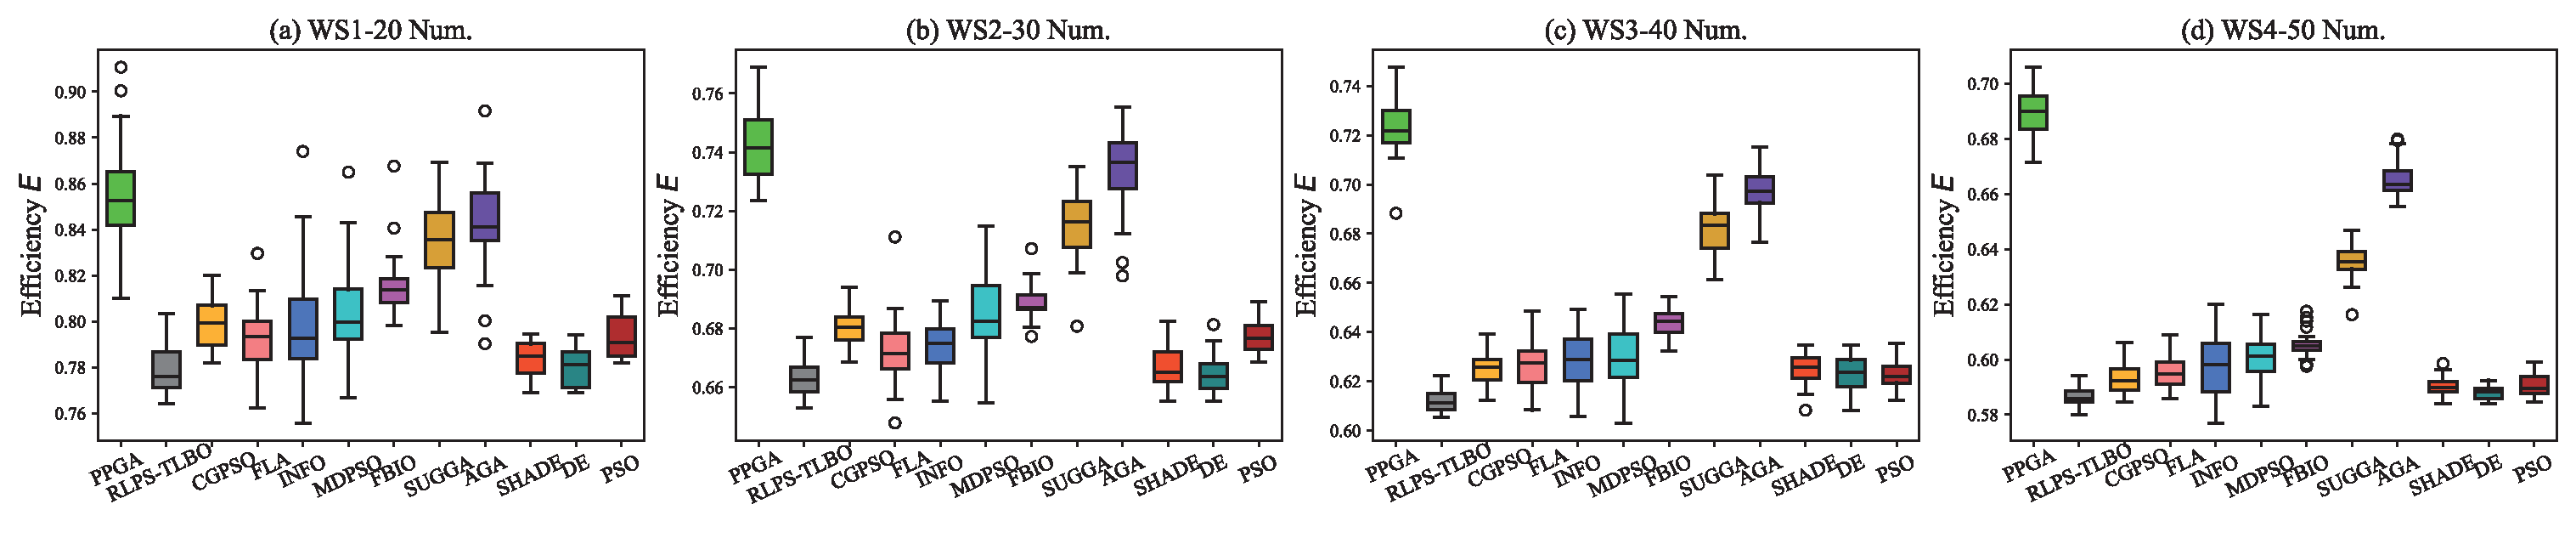
\includegraphics[width=\linewidth,scale=1]{box.eps}
	\caption{Box-whisker-plots of different algorithms under four representative experimental conditions.}
	\label{box}
\end{figure*}

\begin{figure}[!t]\color{blue}
	\centering
	%\setlength{\abovecaptionskip}{-0.2cm}
	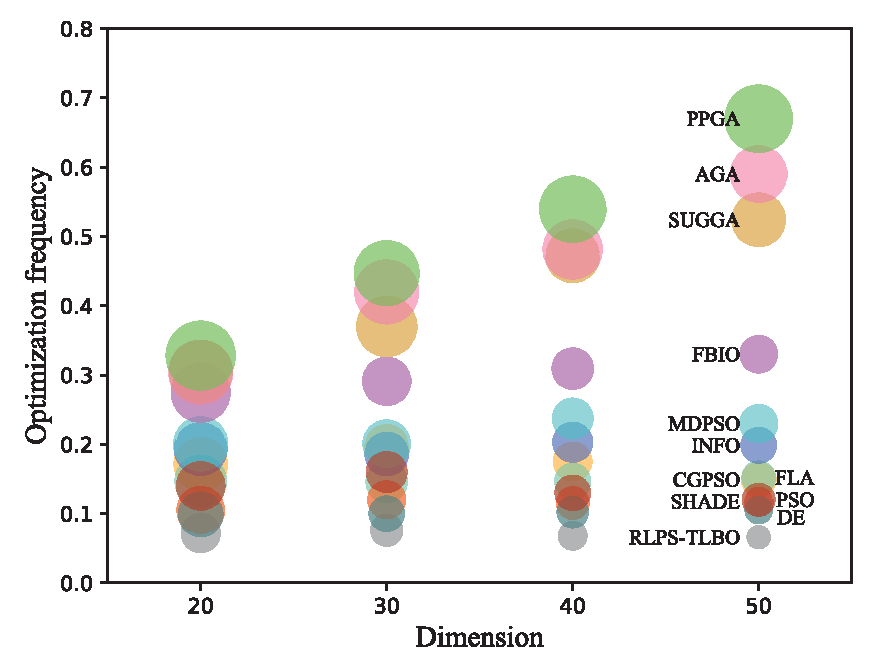
\includegraphics[width=\linewidth,scale=1]{scatter_plot.eps}
	\caption{Scatter-plot of optimization frequency and improvement degree.}
	\label{frequency}
\end{figure}

\begin{figure}[!t]
	\centering
	%\setlength{\abovecaptionskip}{-0.2cm}
	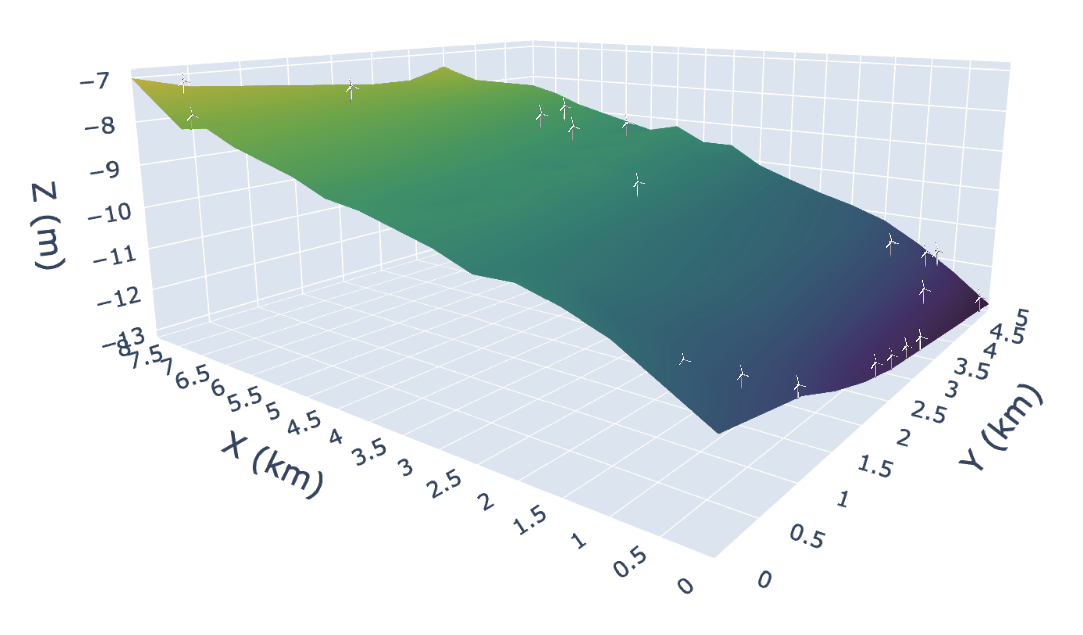
\includegraphics[width=\linewidth,scale=1]{dixing_wt.eps}
	\caption{Optimal layout for 3D simulation given by PPGA in WS1-20 Num.}
	\label{dixing}
\end{figure}
The convergence curve of PPGA demonstrates its superiority over other algorithms in several aspects, including convergence speed, consistency, final solution quality. Fig.~\ref{conv} reveals the convergence trend charts of different algorithms under varying conditions. First, PPGA exhibits a faster convergence rate in the early iterations, indicating its ability to quickly find a near-optimal solution and significantly reduce optimization time. Second, in the middle and later iterations, PPGA's convergence curve is smoother, indicating its stability in fine-tuning the optimization after finding a relatively optimal solution, thus avoiding stagnation in local optima. Moreover, PPGA consistently shows excellent performance under different wind conditions, with the endpoints of its convergence curves significantly higher than those of other algorithms, indicating a higher final energy conversion efficiency. \textcolor{blue}{As the number of wind turbines increases, the performance gap between PPGA and other algorithms becomes increasingly pronounced. While competing algorithms tend to stagnate and cease making significant progress, PPGA continues to actively explore the solution space, persistently seeking improved solutions.} Overall, PPGA achieves higher efficiency and effectiveness in wind farm layout optimization through rapid convergence and stable optimization, demonstrating robustness in high-dimensional environments.

The box-whisker-plots analysis of PPGA is shown in Fig.~\ref{box}, reveals its superior robustness and stability compared to other algorithms. The interquartile range of PPGA is narrower, indicating that the spread of the data points around the median is smaller, and thus, the algorithm's performance is more consistent. A narrower interquartile range also implies that PPGA is less sensitive to variations in initial conditions or random factors, maintaining steady performance across different runs. Additionally, PPGA shows fewer outliers, which signifies its ability to maintain stable results across different runs and conditions. This ability suggests that PPGA is more reliable in real-world applications where stability is crucial. The median performance of PPGA is also higher than that of the other algorithms, demonstrating its effectiveness in achieving better optimization results. These factors collectively highlight PPGA's robust and stable performance in wind farm layout optimization, making it a reliable choice for handling this problem.

To further validate whether PPGA has an advantage in solving this high-dimensional discrete optimization problem, we track the optimization frequency and improvement degree throughout the process. Optimization frequency refers to the proportion of iterations in which the algorithm achieves an improvement, offering insight into the algorithm's vitality and whether it stagnates. Improvement degree reflects the maximum optimization gain that the algorithm can achieve. Fig.~\ref{frequency} presents a scatter-plot showing the performance of different algorithms as the number of turbines increases and the problem dimension grows. The horizontal axis represents the problem dimension, the vertical axis denotes optimization frequency, and the size of the dots indicates the improvement degree. \textcolor{blue}{As the number of turbines increases, the improvement degree of other algorithms decreases, while PPGA maintains nearly the same level of improvement degree. The optimization frequency of PPGA continues to rise, further amplifying its advantage over other algorithms. This highlights the effectiveness of power-law perturbations in sustaining the algorithm's vitality and preventing it from being trapped in local optima.} When faced with high-dimensional optimization scenarios, PPGA consistently achieves stable results and demonstrates remarkable search adaptability.

In this wind farm, spanning an area of 5 km by 8 km with an elevation difference of 6 m, there are 16$\times$27 optimizable positions arranged with a safe spacing of 300 m between turbines. Fig.~\ref{dixing} visually represents the recommended positions of deploying 20 wind turbines using the PPGA algorithm under WS1.

\begin{figure}[t!]
	\centering
	\begin{minipage}{0.45\textwidth}
		\centering
		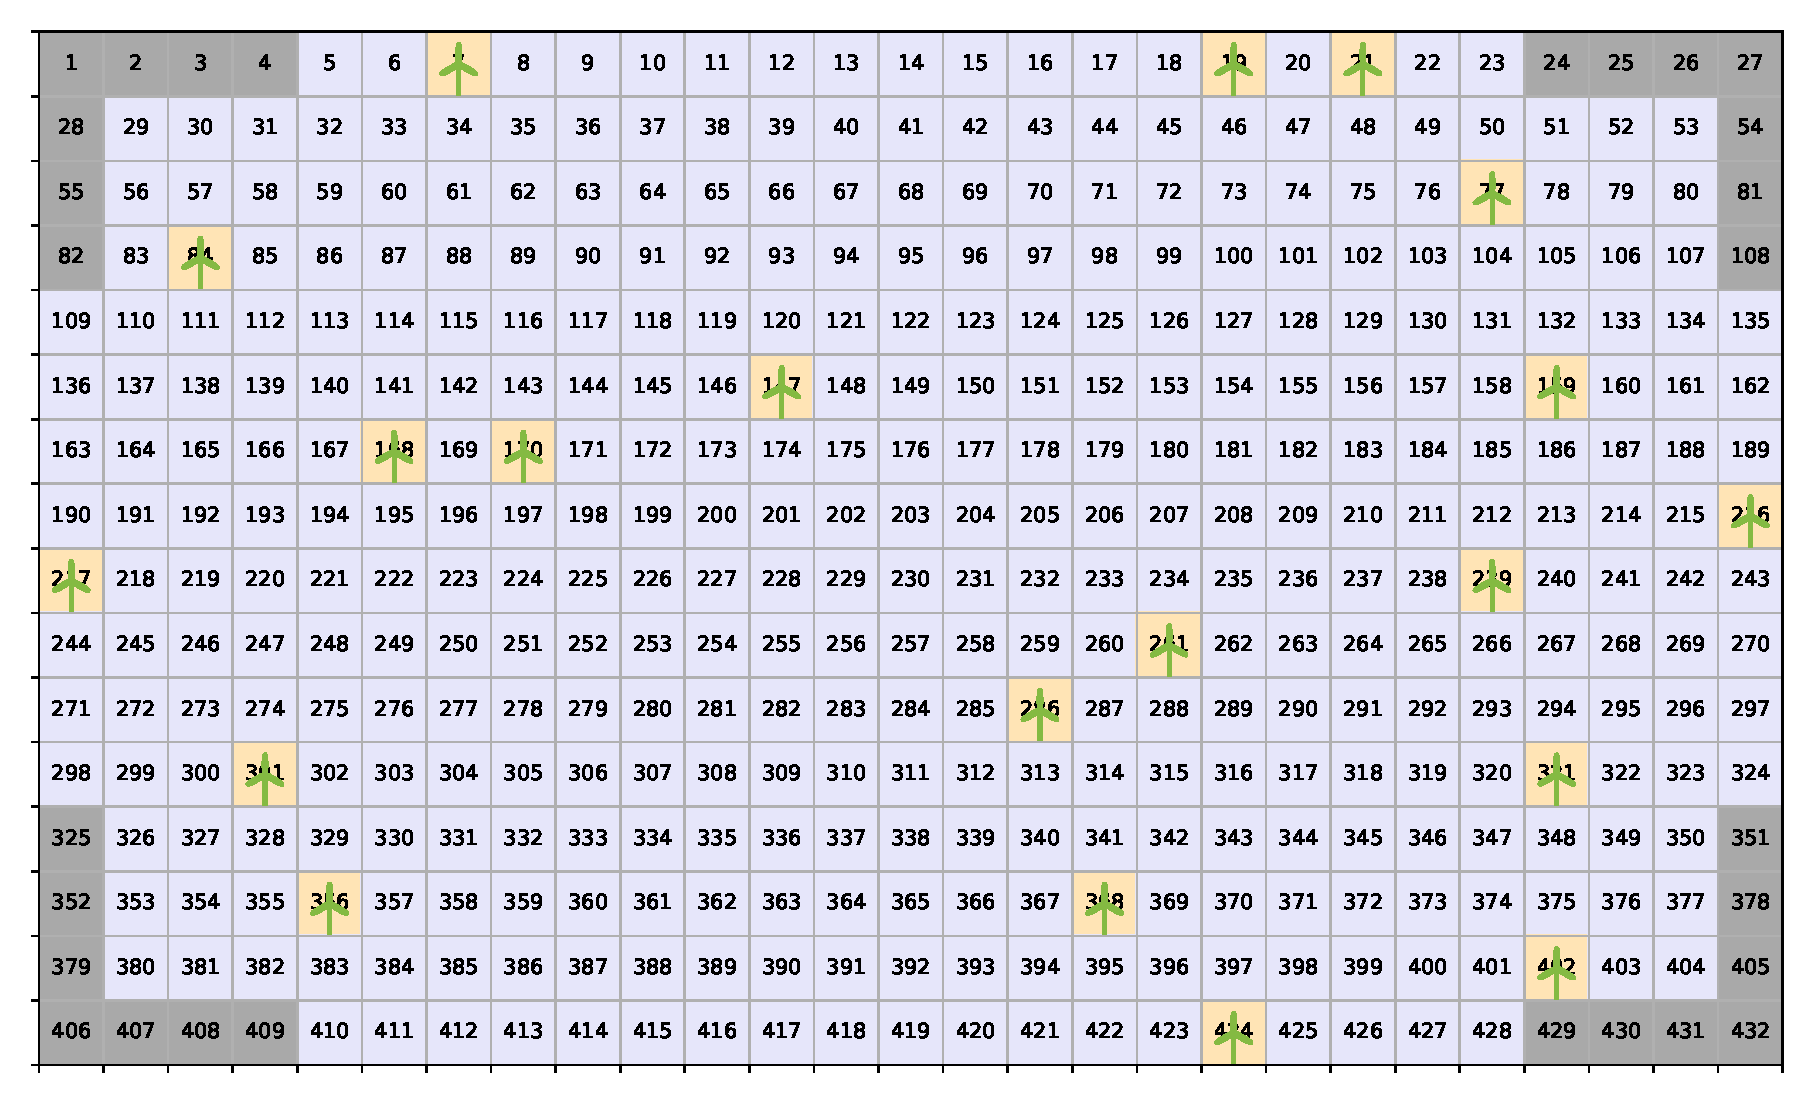
\includegraphics[width=\textwidth]{c1.eps}
		\text{\scriptsize (a) C1 Boundary constraint} % 
	\end{minipage}
	\begin{minipage}{0.45\textwidth}
		\centering
		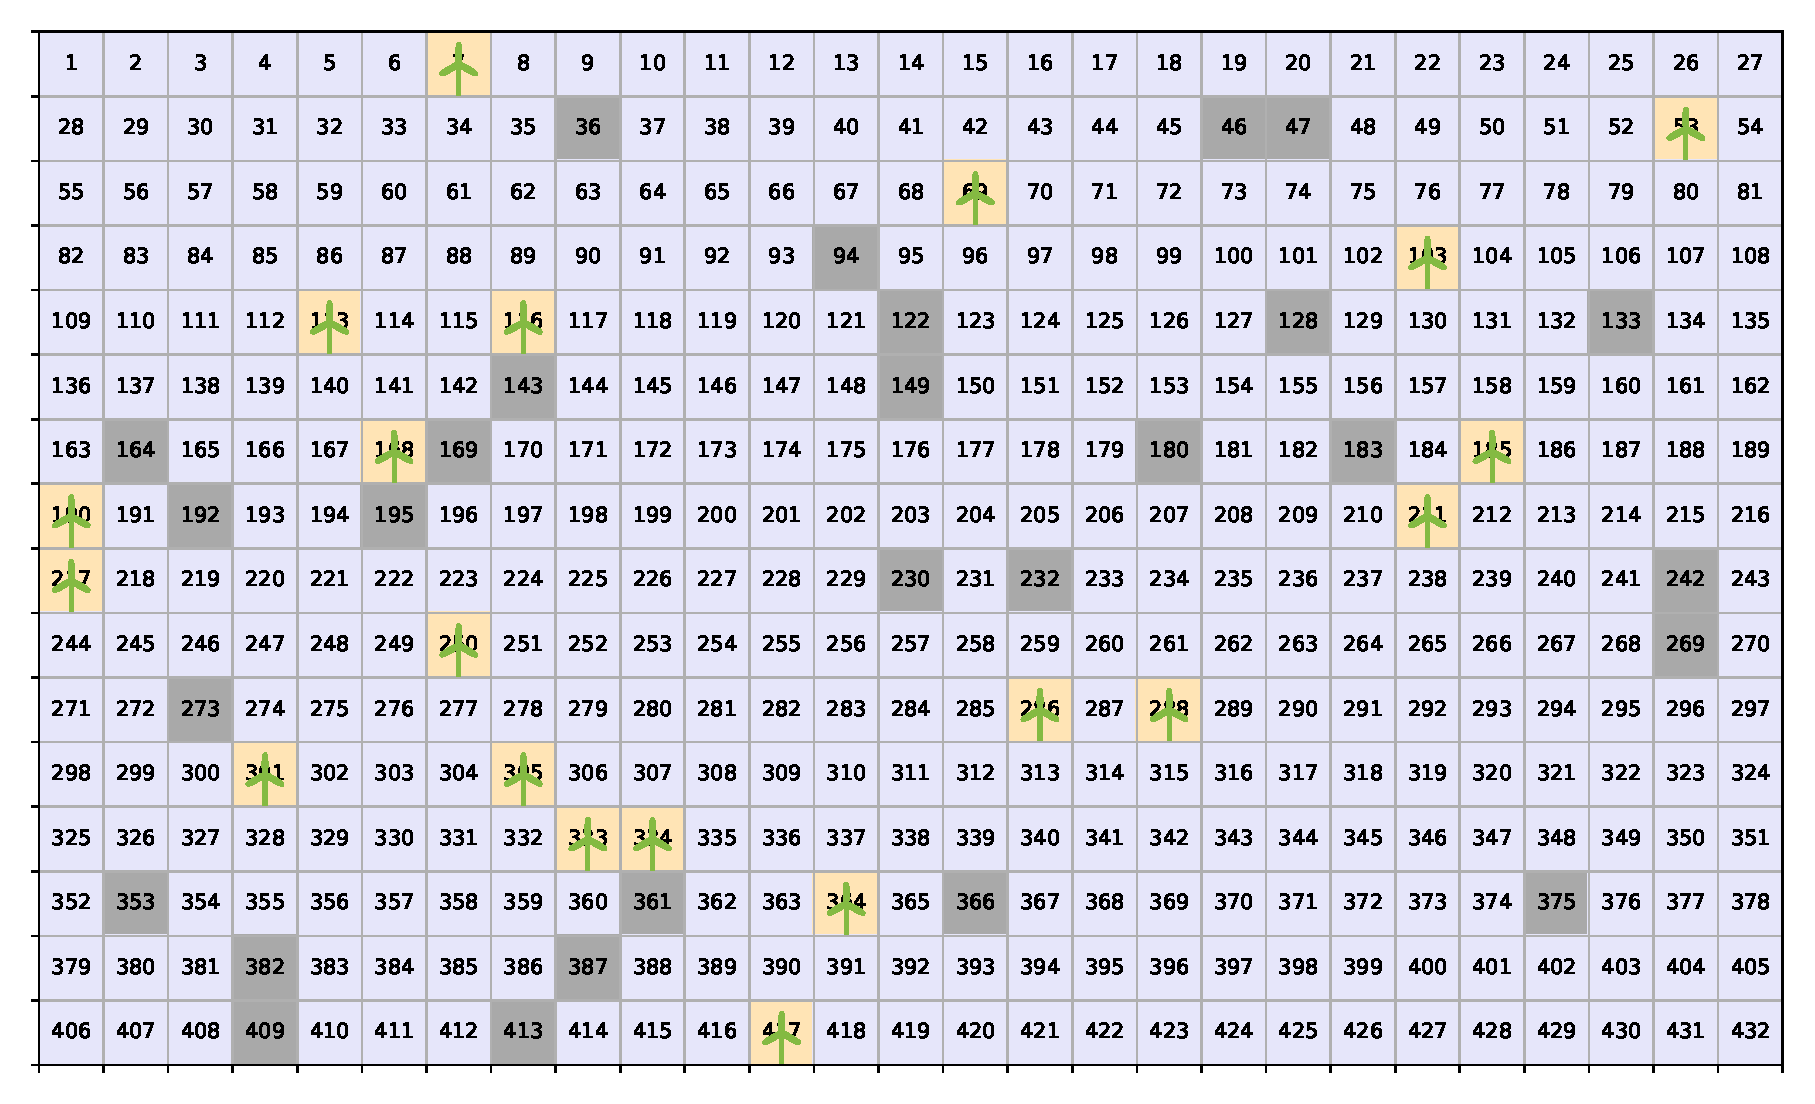
\includegraphics[width=\textwidth]{c2.eps}
		\text{\scriptsize (b) C2 Random constraint} % 
	\end{minipage}
	\caption{Layouts considering boundary constraint and random constraint from obstacles.}
	\label{constraint}
\end{figure}

\begin{table*}[t!]\color{blue}
	\centering
	\caption{The optimal $E$ for different experimental conditions under two constraints.}
	\label{constraintresults}
	\setlength\tabcolsep{4pt}{
	\begin{tabular}{ccccccccccccc} \hline
		& PPGA 	     &	RLPS-TLBO		 &	CGPSO		 &	FLA		&	INFO		&	MDPSO		&	FBIO		&	SUGGA	& AGA & SHADE & DE & PSO \\	\hline
		WS1-C1 20 Num.   &	\textbf{83.23}   &	76.05 +  &	77.93 +  & 77.81 +  & 78.06 + & 78.75 + & 80.12 + & 81.56 + & 82.73 + & 76.82 + & 76.39 + &	77.62 + \\ \hline 
		WS2-C1 30 Num. &	\textbf{72.90}	 &	65.08 +  &	66.42 +	 & 66.10 +	& 66.32 + & 67.24 + & 67.35 + & 70.01 + & 71.53 + & 64.53 + & 64.27 + &	66.03 +	\\ \hline
		WS3-C1 40 Num.  &	\textbf{70.10}	 &	60.01 +	 &	61.23 +	 & 61.56 +	& 61.54 + & 61.68 + & 62.89 + & 66.88 + & 68.40 + & 61.23 + & 60.89 + &	60.96 +	\\ \hline
		WS4-C1 50 Num. &	\textbf{67.22}	 &	56.92 +	 &	57.24 +	 & 58.04 +	& 57.88 + & 58.24 + & 58.72 + & 61.37 + & 64.21 + & 57.08 + & 56.68 + &	56.94 +	\\ \hline
		WS1-C2 20 Num.  &	\textbf{85.32}	 &	77.23 +	 &	78.90 +	 & 79.10 +	& 78.78 + & 80.02 + & 80.79 + & 82.36 + & 83.34 + & 77.21 + & 77.02 + &	78.43 +	\\ \hline
		WS2-C2 30 Num. &	\textbf{73.12}	 &	65.24 +	 &	66.88 +	 & 66.30 +	& 66.48 + & 67.92 + & 68.24 + & 70.95 + & 72.86 + & 65.48 + & 65.07 + &	66.58 +	\\ \hline
		WS3-C2 40 Num.  &	\textbf{71.28}	 &	60.21 +	 &	61.60 +	 & 61.78 +	& 61.94 + & 62.01 + & 63.21 + & 67.25 + & 68.91 + & 61.20 + & 60.96 + &	61.23 +	\\ \hline
		WS4-C2 50 Num.  &	\textbf{68.10}	 &	57.54 +	 &	58.21 +	 & 58.60 +	& 58.81 + & 59.22 + & 59.38 + & 62.14 + & 64.98 + & 58.02 + & 57.82 + &	57.97 +	\\ \hline
	\end{tabular}}
\end{table*}

\begin{table*}[t!]
	\centering
	\caption{The Friedman analysis of parameter $\theta$.}
	\label{ablation}
	\begin{tabular}{cccccccccccc} \hline
		\diagbox{Score}{$\theta$} & -1  & -0.5 & -0.2 & -0.1 & -0.05 & 0 & 0.05 & 0.1 & 0.2 & 0.5 & 1 \\	\hline
		4WS-20 Num.     &	1.59 &	1.64 &	1.82  &	1.91 & 2.09	& 2.91 & 2.32 & 2.64 & 2.27 & 2.18 & 1.64 \\	 \hline
		4WS-30 Num.     &	1.64 &	1.36 &	1.45  &	2.27 & 2.64	& 3.00 & 2.82 & 2.55 & 2.73 & 2.27 & 1.27 \\	 \hline
		4WS-40 Num.     &	1.82 &	1.45 &	1.73  &	1.64 & 1.64	& 3.09 & 2.55 & 3.09 & 2.18 & 2.64 & 2.18 \\	 \hline
		4WS-50 Num.     &	2.18 &	1.18 &	1.82  &	2.09 & 2.18	& 3.18 & 3.00 & 2.55 & 1.82 & 2.09 & 1.91 \\	 \hline
		Total Score   &	7.23 &	5.63 &	6.82  &	7.91 & 8.55	& 12.18 & 10.69 & 10.83 & 9.00 & 9.18 & 7.00 \\\hline
		Rank	 &	8	 &	11	 &	10	 & 7	& 6 & 1 & 3 & 2 & 5 & 4 & 9 	\\ \hline
	\end{tabular}
\end{table*}
\subsection{Constraint Analysis}
In the real world, it is also necessary to consider the potential presence of natural obstacles or artificial obstacles in the region. These obstacles not only restrict the placement of wind turbines but also affect the distribution of wind energy resources and the wake effects within the wind farm. Therefore, failing to adequately account for these constraints may result in layout plans that are impractical in reality or even increase project costs. By incorporating these constraints, the feasibility and reliability of the layout plan can be enhanced, enabling a better balance between technical feasibility and economic efficiency.

Two types of constraint are considered in this study, as illustrated in Fig.~\ref{constraint}: (1) boundary constraint and (2) random constraint. To verify PPGA's ability to handle these two types of constraint, we design 8 representative experimental control groups, considering combinations of different wind conditions, varying numbers of wind turbines, and diverse constraints. The experimental results are shown in Table \ref{constraintresults}. Due to the constraints, the reduced number of feasible layouts leads to a decrease in overall energy conversion efficiency. In all scenarios, PPGA consistently achieves significant improvements and delivers the best optimization results. This highlights PPGA's capability to handle complex experimental conditions with remarkable robustness.

\subsection{Parameter Analysis}
From the previous experimental results and analysis, the power-law perturbation guided by evolutionary fitness has injected powerful momentum into the algorithm's ability to find optimal solutions and continue optimization. Theoretically, the evolutionary fitness index ranges from -1 to 1, though in practice, the algorithm rarely reaches these boundary values. According to (\ref{E14}), values closer to -1 indicate that the population is closer to stagnation and loss of diversity, while values closer to 1 indicate that solution quality and diversity remain high and continue to evolve. Our objective is to determine the optimal perturbation probability. Therefore, we conduct an ablation study to select the best threshold value for deciding the most appropriate perturbation probability. To verify whether this parameter is sensitive to experimental conditions and other factors, we conduct experiments with 11 $\theta$ values under 16 experimental conditions. Table \ref{ablation} shows the Friedman scores and ranking \cite{10460144} of PPGA's performance under different $\theta$ values and experimental conditions.

4WS-20 Num. represents the overall Friedman scores of different $\theta$ values under the condition of 20 turbines and four wind scenarios. From the horizontal scores of each $\theta$, the scores and rankings under different experimental conditions show consistency. This indicates that the parameter is insensitive to different initial conditions and demonstrates good robustness. According to the ranking, $\theta=0$ achieves the highest score and first place. This best parameter is used in all the previous comparison experiments. The distribution of the rankings also shows that the algorithm gets higher scores and rankings when $\theta$ is between 0 and 1. This suggests that power-law perturbation of some of the inferior individuals is an effective incentive. When $\theta=0$, 0.05 and 0.5, the top three rankings are achieved, indicating that the probability of applying power-law perturbations to the population is optimal at these thresholds. Excessive and inappropriate perturbations degrade the performance of the algorithm when $\theta$ is close to 1, which underscores that the key to enhancing the search capability of the algorithm lies in applying suitable incentive strategies at the right moments.

\subsection{Discussion}
Traditional 2D wind farm optimization models often overlook two critical factors: 1) the impact of terrain undulations and altitude variations on wind speed and direction and 2) the complex wake effects between turbines under real-world conditions. Motivated by these challenges, we have developed a 3D wind farm optimization model that incorporates altitude, utilizing a 3D wake model to more accurately reflect real conditions. This allows for more precise simulation of wind flow under various terrain conditions, leading to better predictions of how each turbine's position affects the overall performance of the wind farm.

To address the optimization complexity in high-dimensional discrete environments and to overcome common issues of local optima and optimization stagnation, we propose an evolutionary adaptation degree-guided genetic algorithm based on power-law perturbation. This algorithm not only adapts to multidimensional conditions but also effectively avoids premature convergence and local optima by introducing power-law perturbations, thereby enhancing global search capabilities and optimization results.

To support our claims and demonstrate the effectiveness of PPGA, we conduct extensive experiments. The previous experimental results have shown that PPGA achieves excellent performance in complex high-dimensional wind farm optimization problems. This includes the accuracy of turbine layout and the overall improvement in wind energy utilization efficiency.

However, the proposed PPGA has certain limitations: 1) The computational cost of evolutionary adaptation degree and power-law perturbations, especially in very large populations, can be resource-intensive. 2) The algorithm's performance relies on the correct tuning of perturbation probabilities, which may vary significantly across different scenarios and datasets. These limitations can be mitigated by developing more efficient perturbation mechanisms to reduce computational overhead without sacrificing optimization quality, and implementing tuning strategies based on real-time feedback from the optimization process to ensure the algorithm remains effective under various conditions. \textcolor{blue}{Furthermore, integrating deep network models and learning strategies may help the algorithm learn patterns and relationships from complex data adaptively \cite{8948246}. For example, reinforcement learning can dynamically adjust parameters based on the optimization state to guide the exploration process, while neural networks can identify and predict promising solution regions, thereby improving both efficiency and robustness \cite{9043894,9426596}.}

In addition, we observe that as the number of wind turbines reaches a certain level, the conversion efficiency of the total output decreases very slowly during the experiments, indicating a form of stagnation. As the number of turbines increases, the distance between them shortened, and the wake effect between the turbines become more significant. The wake effect results in downstream turbines receiving reduced wind speeds, thereby decreasing the overall efficiency of the wind farm \cite{9930666}. The results revealed by Tables \ref{WS1} $-$ \ref{WS4} show the rate of efficiency decline gradually slows down as the quantity increases. This indicates that the impact of the wake effect becomes unavoidable, and the optimizable spatial positions rapidly decrease. Further improving this model and enhancing its efficiency decline curve is one of the key focus areas of our work.

\textcolor{blue}{Furthermore, large-scale and ultra-large-scale wind farm optimization presents a significant challenge in this field. The adoption of a three-dimensional wake model causes computational costs to rise significantly as the number of turbines increases, leading to extremely time-consuming wake calculations. As the wind farm size grows, the interactions between turbines become increasingly intricate, which further exacerbates the computational burden. Developing methods to simplify the computational framework, while maintaining the accuracy of the wake models, is one of the key focus areas of our work.}

In summary, by combining advanced 3D modeling and innovative algorithmic strategies, we aim to provide a robust and scalable solution to enhance wind farm efficiency and promote the development of renewable energy technologies.	
\section{Conclusion}
\label{sec_conclusion}
In this paper, we propose an evolutionary adaptation degree-guided genetic algorithm based on power-law perturbation~(PPGA) to address the complex wind farm layout optimization. In addition, we construct a 3D wind farm layout modeling framework using a high-fidelity wake model. Utilizing the topography and wind data of the Nantong wind power project along the southeastern coast as a case study, PPGA is compared with various algorithms that perform well on this problem under different conditions. The proposed PPGA achieves the highest energy output and conversion rates. This study provides references and experiences for the future development of wind power along the southeast coast of China.
 
The further direction can focus on the following three aspects: 1) Improve the wind energy macro model by integrating terrain constraints, heterogeneous wind turbines, and other factors into a comprehensive optimization framework. \textcolor{blue}{2) Address the challenge of high computational costs in large-scale wind farm optimization by developing efficient approximate calculation methods. 3) Develop more promising optimization algorithms, such as embedding learning networks to overcome the inherent shortcomings of tradition algorithms.}    

\bibliographystyle{IEEEtran}
\bibliography{mybibfile}

\end{document}
